\documentclass[fontset=none,11pt,a4paper,fleqn]{ctexart}
\usepackage{fontspec}
\IfFontExistsTF{Times New Roman}{\setmainfont{Times New Roman}}{\setmainfont{Liberation Serif}}
\IfFontExistsTF{Liberation Sans}{\setsansfont{Liberation Sans}}{}
\IfFontExistsTF{SimSun}{\setCJKmainfont{SimSun}[AutoFakeBold=2]}{\setCJKmainfont{Noto Serif CJK SC}}
\IfFontExistsTF{Microsoft YaHei}{\setCJKsansfont{Microsoft YaHei}}{\setCJKsansfont{SimHei}}
\usepackage{amsmath,amsthm}
\usepackage{unicode-math}
\IfFontExistsTF{TeX Gyre Termes Math}{\setmathfont{TeX Gyre Termes Math}}{\setmathfont{latinmodern-math.otf}}
\usepackage[a4paper,margin=0.9in]{geometry}
\usepackage[authoryear,round]{natbib}
\usepackage{booktabs,longtable,array,tabularx}
\usepackage{microtype}
\usepackage{xcolor}
\usepackage{enumitem}
\usepackage{placeins}
\usepackage{graphicx}
\usepackage{needspace}
\usepackage{xurl}
\usepackage[skins,breakable]{tcolorbox}
\usepackage{tikz}
\usetikzlibrary{arrows.meta,positioning,calc}
\usepackage[hidelinks,unicode=true]{hyperref}
\usepackage{caption}
\captionsetup{font=small,labelfont=normalfont,textfont=normalfont,labelsep=quad,skip=6pt}
\captionsetup[figure]{name=图}
\captionsetup[table]{name=表}

\setlength{\mathindent}{2em}
\numberwithin{equation}{section}
\setlength{\parskip}{0.25ex plus 0.15ex}
\linespread{1.12}
\pagestyle{plain}

\ctexset{
  section={
    format=\normalfont\large\bfseries\raggedright,% qa-allow-bold
    name={,.},
    aftername=\enspace,
    beforeskip={3.0ex plus 1ex minus .2ex},
    afterskip={1.5ex plus .2ex}
  },
  subsection={
    format=\normalfont\normalsize\bfseries\raggedright,% qa-allow-bold
    name={,.},
    aftername=\enspace,
    beforeskip={2.2ex plus 1ex minus .2ex},
    afterskip={1.0ex plus .2ex}
  }
}

\definecolor{boxbg}{RGB}{245,247,250}
\definecolor{boxrule}{RGB}{120,138,165}
\definecolor{boxhead}{RGB}{70,88,118}
\definecolor{notefg}{RGB}{78,84,94}

% 原公式与来源框：全文统一样式
\newtcolorbox{yuan}[1][原公式与来源]{enhanced,breakable,
  colback=boxbg,colframe=boxbg,boxrule=0pt,
  borderline west={1.2pt}{0pt}{boxrule},
  sharp corners,left=8pt,right=6pt,top=4pt,bottom=4pt,
  before skip=6pt,after skip=6pt,
  fontupper=\small,
  title={\textsf{#1}},
  coltitle=boxhead,colbacktitle=boxbg,
  attach title to upper,after title={\enspace}}

% 推导步骤的注：全文统一样式
\newcommand{\zhu}[1]{\par\nopagebreak\vspace{1pt}%
  {\small\color{notefg}\textsf{注}\enspace #1\par}}

\newtheoremstyle{zhthm}{1.0ex}{0.8ex}{\normalfont}{}{\sffamily}{}{0.8em}%
  {\thmname{#1}\thmnumber{ #2}\thmnote{\enspace（#3）}}
\newtheoremstyle{zhrem}{0.8ex}{0.8ex}{\normalfont}{}{\sffamily\color{boxhead}}{}{0.8em}%
  {\thmname{#1}\thmnumber{ #2}\thmnote{\enspace（#3）}}
\theoremstyle{zhthm}
\newtheorem{definition}{定义}[section]
\newtheorem{lemma}[definition]{引理}
\newtheorem{proposition}{命题}
\newtheorem{corollary}{推论}
\theoremstyle{zhrem}
\newtheorem*{conditions}{适用条件}

\makeatletter
\renewenvironment{proof}[1][证明]{\par\pushQED{\qed}\normalfont
  \topsep4pt\relax\trivlist\item[\hskip\labelsep\sffamily #1\hspace{0.8em}]%
  \@ifnextchar\begin{\leavevmode\par\vspace{-0.8ex}}{\ignorespaces}}%
  {\popQED\endtrivlist\@endpefalse}
\makeatother

\setlist[enumerate]{label=\arabic*.,leftmargin=1.8em,itemsep=0.5ex,topsep=0.6ex}
\setlist[itemize]{leftmargin=1.8em,itemsep=0.3ex,topsep=0.5ex}

\newcommand{\E}{\mathbb{E}}
\newcommand{\Var}{\operatorname{Var}}
\newcommand{\Cov}{\operatorname{Cov}}
\newcommand{\Corr}{\operatorname{Corr}}
\newcommand{\Rbar}{\bar R}
\newcommand{\NB}{\mathrm{NB}}
\newcommand{\Bin}{\mathrm{Bin}}
\newcommand{\mx}{m_{\times}}
\newcommand{\Rhat}{\hat R}
\newcommand{\CV}{\mathrm{CV}}
\newcommand{\ptag}[1]{\tag*{论文 (#1)}}

\title{疫情再生数监测精度极限的理论推导\\[0.4ex]
  {\large 与《环境随机性与不完全报告下疫情再生数监测的精度极限与优化设计》\\
  第 2 节及附录 A--C 逐式对照}}
\author{}
\date{}

\begin{document}
\maketitle
\thispagestyle{plain}
\vspace{-6ex}

\section{阅读指南与记号}\label{sec:guide}

本文逐式展开论文第 2 节（模型与方法）与附录 A--C 的理论结果，供与论文对照阅读。各结果采用统一体例。命题、推论或引理先陈述论文中的结论，并在括号中标出论文编号；随后的浅色框列出推导所依赖的原公式及其出处，凡取自他人论文或教材的结果注明文献与原文位置，原文式号未经核对的只引文献；证明逐步写出，每步之后以“注”说明所用公式；最后列出适用条件，论文未写明的前提单独标出，并汇总于第~\ref{sec:errata}~节。

编号规则如下。本文自身的式子按节编号，如 (4.1)；预备公式编为 (P1)--(P13)；转录自论文的式子在右侧标注论文式号，如“论文 (A.3)”指论文附录式 (A.3)。命题 1--4 与推论 1--2 沿用论文编号，定义与引理按节编号。附录中原无编号的式子按论文排版顺序编号。表~\ref{tab:map}~给出论文对象与本文位置的对应，表~\ref{tab:notation}~为记号表，图~\ref{fig:dep}~给出假设、引理与命题之间的依赖关系。

文中数值所用的基线参数为
\begin{equation}\label{eq:baseline}
\Rbar=1.15,\qquad v_R=0.04,\qquad k=0.35,\qquad \rho=0.25,\qquad \tau=0.15,
\end{equation}
“代入基线值”均指代入式~\eqref{eq:baseline}。由此得 $\Rbar^2+v_R=1.3625$。

\begin{small}
\setlength{\tabcolsep}{5pt}
\renewcommand{\arraystretch}{1.12}
\begin{longtable}{@{}p{0.25\linewidth}p{0.36\linewidth}p{0.33\linewidth}@{}}
\caption{论文对象与本文位置的对应。论文位置一栏给出论文中的节号与式号，本文位置一栏给出对应的命题、引理与节号。}\label{tab:map}\\
\toprule
论文对象 & 论文位置 & 本文位置 \\
\midrule
\endfirsthead
\multicolumn{3}{@{}l}{\small 表~\ref{tab:map}（续）}\\
\toprule
论文对象 & 论文位置 & 本文位置 \\
\midrule
\endhead
\bottomrule
\endfoot
后代分布 & 第 2.1 节，式 (1) & 引理~\ref{lem:offspring}，第~\ref{sec:model}~节 \\
报告病例数分布 & 第 2.1 节，式 (2)；附录 A.1 & 引理~\ref{lem:cases} \\
误差分解 & 第 2.1 节，式 (3) & 引理~\ref{lem:decomp} \\
似然、得分与 UMVUE & 附录 A.2，式 (A.1)、(A.2) & 引理~\ref{lem:umvue} \\
命题 1 & 第 2.2 节，式 (4)；附录 A.3，式 (A.3)--(A.5) & 命题~\ref{prop:1}，第~\ref{sec:prop1}~节 \\
自相关环境的预测误差 & 第 2.2 节 & 引理~\ref{lem:ar1} \\
多辖区汇总 & 第 2.2 节，式 (5) & 引理~\ref{lem:pool} \\
命题 2 & 第 2.3 节，式 (6)；附录 A.4，式 (A.6)、(A.7) & 命题~\ref{prop:2}，第~\ref{sec:prop2}~节 \\
命题 3 & 第 2.3 节，式 (7)--(9)；附录 A.5，式 (A.8)--(A.10) & 命题~\ref{prop:3}、引理~\ref{lem:S}--\ref{lem:rho}，第~\ref{sec:prop3}~节 \\
表 S7 三项分解 & 表 S7；结果第 3.1 节 & 引理~\ref{lem:s7} \\
推论 1 & 第 2.3 节，式 (10)；附录 A.6，式 (A.11)、(A.12) & 推论~\ref{cor:1}，第~\ref{sec:cor1}~节 \\
加权增长比与更新型比值 & 第 2.5 节，式 (11)、(12) & 定义~\ref{def:G}、引理~\ref{lem:RA} \\
更新方程下的预测方差 & 第 2.5 节，式 (13)；附录 A.7，式 (A.13) & 引理~\ref{lem:eq13} \\
仿射损失与潜在平衡规模 & 第 2.6 节，式 (14)；附录 B.2 & 引理~\ref{lem:affine} \\
分母二项噪声 & 第 2.6 节，式 (15)；附录 A.7，式 (A.14) & 引理~\ref{lem:eq15} \\
共享报告冲击 & 附录 B.1，式 (B.1)--(B.6) & 引理~\ref{lem:B3}--\ref{lem:B6}，第~\ref{sec:shock}~节 \\
等效界尺度与功效 & 附录 B.3；第 2.8 节 & 引理~\ref{lem:B7}、\ref{lem:tost} \\
FGLS、双向聚类自助 & 第 2.7 节 & 第~\ref{sec:fgls}--\ref{sec:boot}~节 \\
季间合并与区间 & 第 2.9 节 & 第~\ref{sec:dl}--\ref{sec:tint}~节 \\
命题 4 & 附录 C.1，式 (C.1) & 命题~\ref{prop:4}，第~\ref{sec:ext}~节 \\
自相关环境的预算分配 & 附录 C.2，式 (C.2)、(C.3) & 引理~\ref{lem:C2} \\
推论 2 & 附录 C.3 & 推论~\ref{cor:2} \\
检验 $R_t>1$ 的一致最优性 & 附录 C.4 & 引理~\ref{lem:ump} \\
收缩估计 & 附录 C.5，式 (C.4) & 引理~\ref{lem:shrink} \\
表 S7 各汇总量 & 表 S7 & $V,\mx$：命题~\ref{prop:1}；$V_H,m_{\times,H}$：命题~\ref{prop:2}；$m^*,S,\rho^*$：第~\ref{sec:prop3}~节；$T^\dagger,\mathcal B^\dagger$：引理~\ref{lem:C2} \\
\end{longtable}
\end{small}

\begin{longtable}{@{}p{0.2\linewidth}p{0.52\linewidth}p{0.2\linewidth}@{}}
\caption{记号表。首次出现一栏指论文中的位置。}\label{tab:notation}\\
\toprule
记号 & 含义 & 首次出现 \\
\midrule
\endfirsthead
\multicolumn{3}{@{}l}{\small 表~\ref{tab:notation}（续）}\\
\toprule
记号 & 含义 & 首次出现 \\
\midrule
\endhead
\bottomrule
\endfoot
$t$ & 时期（一代或一周）索引 & 第 2.1 节 \\
$n$ & 原发病例数，即一代中的父代人数 & 式 (1) \\
$X_{i,t}$ & 第 $i$ 名原发病例产生的继发感染数（后代数） & 式 (1) \\
$R_t$ & 瞬时再生数，即给定时期 $t$ 时每名感染者的期望后代数 & 式 (1) \\
$k$ & 负二项离散参数；$k$ 越小，传播越集中于少数感染者 & 式 (1) \\
$\rho$ & 每例感染被报告的概率（报告完整度） & 式 (2) \\
$C_t$ & 报告病例数 & 式 (2) \\
$m=\rho n$ & 病例量，即 $R_t=1$ 时每期期望报告数 & 式 (2) 之后 \\
$\Rhat_t=C_t/m$ & 尺度化病例数 & 式 (3) \\
$\Rbar,\ v_R$ & $R_t$ 跨时期的均值与方差（环境变异） & 第 2.1 节 \\
$U=\Rbar^2+v_R$ & $\E {R_t}^2$ & 附录 A.3 \\
$A=\Rbar+\rho U/k$ & 抽样方差系数 & 式 (4) \\
$\mx=A/v_R$ & 理论平衡规模 & 命题 1(iii) \\
$p_t,\ \tau$ & 时变报告概率；相对标准差 $\mathrm{SD}(p_t)/\rho$ & 假设 H5 \\
$v_H,\ A_H,\ m_{\times,H}$ & 报告异质性下的附加方差、抽样系数与平衡规模 & 式 (6) \\
$T,\ c_0,\ c_1,\ \mathcal B$ & 时期数、每期固定成本、每例成本、总预算 & 命题 3 \\
$\phi,\ S(\phi,T)$ & $R_t$ 的 AR(1) 系数；相关和 $\sum_{s,t}\phi^{\lvert s-t\rvert}$ & 式 (9) \\
$\psi$ & 报告波动 $p_t/\rho-1$ 的 AR(1) 系数 & 表 S7 \\
$\nu$ & 每期抽样的报告单位数 & 推论 1 \\
$w_j,\ \Lambda_t$ & 代际间隔权重；感染压力 $\sum_jw_jI_{t-j}$ & 式 (13) \\
$\mathcal F_t$ & 截至 $t$ 的历史 & 式 (13) \\
$G_t,\ D_t$ & 加权增长比及其分母 & 式 (11) \\
$R_{A,t},\ r_t$ & 更新型比值与日增长率 & 式 (12) \\
$\alpha,\ \theta$ & 代际间隔伽马分布的形状与尺度 & 式 (12) \\
$M_t,\ L_t$ & 经验规模变量；相对损失 & 式 (14) \\
$a,\ b,\ b/a$ & 仿射损失模型的截距、斜率与表观平衡规模 & 式 (14) \\
$c_w$ & 分母二项噪声系数 $(1-\rho)\sum_j{w_j}^2$ & 式 (A.14) \\
$\varepsilon_t,\ K(t,s)$ & 乘性报告冲击及其条件协方差 & 附录 B.1 \\
$q_{tj},\ u_t,\ y_t$ & 路径权重、分母冲击、无冲击比值 & 式 (B.1) \\
$B_t,\ V_t$ & 二阶偏差系数与方差系数 & 式 (B.3) \\
$\kappa(g)$ & $R_A$ 变换的对数弹性 & 式 (B.6) \\
$\xi=\Rbar^2/v_R$ & 伽马形状参数 & 命题 4 \\
$\psi'$ & 三伽马函数 & 式 (C.1) \\
$\eta_s,\ v_S,\ S$ & 流行季效应、季间方差、季数 & 推论 2 \\
$\NB(r,p)$ & 负二项分布，见定义~\ref{def:nb} & --- \\
\end{longtable}

\begin{figure}[!tbp]
\centering
\begin{tikzpicture}[
  x=0.94cm,
  font=\small,
  hyp/.style={draw=boxrule,fill=boxbg,rounded corners=2pt,align=center,inner sep=3pt,minimum height=2.8em,minimum width=#1},
  hyp/.default=6.6em,
  lem/.style={draw=boxrule,fill=white,rounded corners=2pt,align=center,inner sep=3pt,minimum height=2.8em,minimum width=#1},
  lem/.default=6.6em,
  pro/.style={draw=boxhead,fill=boxbg!40!white,line width=0.8pt,rounded corners=2pt,align=center,inner sep=3pt,minimum height=2.8em,minimum width=#1},
  pro/.default=6.6em,
  ar/.style={-{Stealth[length=4pt]},color=notefg,line width=0.5pt},
  lab/.style={font=\footnotesize\sffamily,color=boxhead,anchor=west}
]
% 第一层：假设
\node[hyp] (H13) at (0,0) {H1--H3\\独立报告与后代};
\node[hyp] (H4) at (3.0,0) {H4\\$n$ 由设计固定};
\node[hyp] (H5) at (6.0,0) {H5\\报告概率时变};
\node[hyp] (Hab) at (9.0,0) {前提 (a)--(e)\\更新方程与分母};
\node[hyp] (Hg) at (12.0,0) {伽马或正态\\环境分布};
% 第二层：引理
\node[lem] (L2) at (0,-2.0) {引理~\ref{lem:cases}\\式 (1)、(2)};
\node[lem] (L3) at (3.0,-2.0) {引理~\ref{lem:decomp}\\式 (3)};
\node[lem] (L4) at (6.0,-2.0) {引理~\ref{lem:umvue}\\UMVUE};
\node[lem] (L13) at (9.0,-2.0) {引理~\ref{lem:eq13}\\式 (13)};
\node[lem] (L15) at (12.0,-2.0) {引理~\ref{lem:eq15}\\式 (15)};
% 第三层：主要结果
\node[pro] (P1) at (0,-4.0) {命题 1\\式 (4)};
\node[pro] (P2) at (3.0,-4.0) {命题 2\\式 (6)};
\node[pro] (C1) at (6.0,-4.0) {推论 1\\式 (10)};
\node[pro] (L14) at (9.0,-4.0) {引理~\ref{lem:affine}\\式 (14)};
\node[pro] (P4) at (12.0,-4.0) {命题 4、推论 2\\附录 C};
% 第四层：设计结果
\node[pro] (P3) at (0,-6.0) {命题 3\\式 (7)--(9)};
\node[pro] (S7) at (3.0,-6.0) {表 S7\\三项分解};
\node[pro] (C2) at (6.0,-6.0) {引理~\ref{lem:C2}\\附录 C.2};
\node[pro] (B) at (9.0,-6.0) {附录 B\\共享冲击};
\node[pro] (Sh) at (12.0,-6.0) {引理~\ref{lem:ump}、\ref{lem:shrink}\\检验与收缩};
% 依赖
\draw[ar] (H13) -- (L2);
\draw[ar] (L2) -- (L3);
\draw[ar] (L2.south east) -- (L4.south west);
\draw[ar] (H13.south east) -- (L4.north west);
\draw[ar] (H4) -- (L3);
\draw[ar] (L3) -- (P1);
\draw[ar] (L4.south) .. controls +(0,-1.2) and +(1.0,0.4) .. (P1.north east);
\draw[ar] (P1) -- (P2);
\draw[ar] (H5) .. controls +(-1.4,-1.2) and +(0.4,1.0) .. (P2.north east);
\draw[ar] (P2) -- (C1);
\draw[ar] (P1) -- (P3);
\draw[ar] (P2) -- (S7);
\draw[ar] (P3) -- (S7);
\draw[ar] (P3.south) .. controls +(0,-0.9) and +(0,-0.9) .. (C2.south);
\draw[ar] (Hab) -- (L13);
\draw[ar] (L2.north east) .. controls +(2.5,0.9) and +(-2.0,0.9) .. (L13.north west);
\draw[ar] (L13) -- (L14);
\draw[ar] (Hab.south east) -- (L15.north west);
\draw[ar] (L15) -- (L14);
\draw[ar] (L14) -- (B);
\draw[ar] (Hg.east) .. controls +(1.0,-1.2) and +(1.0,1.2) .. (P4.east);
\draw[ar] (P4) -- (Sh);
\draw[ar] (L2.south west) .. controls +(-0.45,-1.6) and +(-0.45,0.5) .. (P3.north west);
% 层标签
\node[lab,anchor=east] at (-1.45,0) {假设};
\node[lab,anchor=east] at (-1.45,-2.0) {引理};
\node[lab,anchor=east] at (-1.45,-4.0) {结论};
\node[lab,anchor=east] at (-1.45,-6.0) {设计};
\end{tikzpicture}
\caption{假设、引理与命题之间的依赖关系。箭头由被引用的结果指向使用它的结果；浅色底框为假设，白底框为引理，深色边框为主要结论。}
\label{fig:dep}
\end{figure}

\section{最小背景}\label{sec:background}

\subsection{再生数与后代分布}

传染病在人群中按代传播：一名感染者（原发病例）在其传染期内使若干人感染（继发病例）。时期 $t$ 的瞬时再生数 $R_t$ 定义为每名感染者的期望继发感染数。$R_t>1$ 时感染人数增长，$R_t<1$ 时感染人数下降。

单个感染者的继发感染数称为后代数。不同感染者的传染力差异很大，少数超级传播者造成大部分传播。\citet[正文第 2 段]{lloydsmith2005superspreading} 把个体传染力 $\nu$ 设为均值 $R_0$、形状 $k$ 的伽马变量，给定 $\nu$ 时后代数服从泊松分布，于是后代数服从负二项分布，方差为 $R_0(1+R_0/k)$。$k\to\infty$ 时该分布退化为泊松分布，$k$ 越小，后代数越分散。

\subsection{报告}

监测系统只记录被报告的病例。每例感染独立地以概率 $\rho$ 被报告，等价于对感染数作二项稀疏化。论文的实证部分以住院为报告事件，$\rho$ 即每例感染的住院概率。真实计数与报告概率相乘的层级结构也是漏报计数模型的基本形式 \citep[Sec.~2.2]{stoner2019hierarchical}。

\subsection{代际间隔与更新方程}

感染者感染他人的时刻相对其自身被感染时刻的延迟称为代际间隔，其分布记为 $w$。连续时间的更新方程为
\begin{equation*}
I(t)=\int_{\,(0,\infty)} R(t)\,w(\tau)\,I(t-\tau)\,\mathrm d\tau ,
\end{equation*}
见 \citet[式 (1)、(6)]{fraser2007estimating}。离散形式为 $\E(I_t\mid\text{历史})=R_t\Lambda_t$，其中 $\Lambda_t=\sum_{s\ge1}w_sI_{t-s}$ 称为总传染力或感染压力 \citep[Materials and Methods 第 3、6 段]{cori2013new}。

\subsection{两类随机性}

种群生态学区分两类随机性 \citep{engen1998demographic,lande2003stochastic}。种群统计随机性来自个体层面的独立随机事件，例如每名感染者造成几例继发感染、每例感染是否被报告；其相对影响随规模增大按 $1/m$ 衰减。环境随机性来自同时作用于全体个体的共同冲击，例如湿度、学期与节假日使 $R_t$ 本身在时期之间变化 \citep[引言]{dalziel2018urbanization}；其影响与规模无关。论文的核心结论由此而来：增加病例量只能消除前一类误差，后一类误差构成精度的下限。

\section{预备工具}\label{sec:tools}

本节写出后文反复使用的原始公式，编号为 (P1)--(P13)。

\subsection{负二项分布}

\begin{definition}[负二项分布]\label{def:nb}
设 $r>0$，$p\in(0,1)$。称 $X\sim\NB(r,p)$，若
\begin{equation*}
\Pr(X=x)=\frac{\Gamma(x+r)}{\Gamma(r)\,x!}\,p^{r}(1-p)^{x},\qquad x=0,1,2,\dots
\end{equation*}
\end{definition}

其概率母函数（PGF）为
\begin{equation}
G_X(s)=\E s^X=\left[\frac{p}{1-(1-p)s}\right]^{r},\qquad \lvert s\rvert<\frac{1}{1-p}.
\tag{P1}
\end{equation}
由 $G'(1)=\E X$ 与 $G''(1)=\E X(X-1)$ 得
\begin{equation}
\E X=\frac{r(1-p)}{p},\qquad \Var X=G''(1)+G'(1)-G'(1)^2=\frac{r(1-p)}{p^2}.
\tag{P2}
\end{equation}

\begin{lemma}[可加性]\label{lem:add}
若 $X_1,\dots,X_n$ 独立，$X_i\sim\NB(r_i,p)$，且成功概率 $p$ 相同，则
\begin{equation}
\sum_{i=1}^nX_i\sim\NB\Big(\sum_{i=1}^nr_i,\ p\Big).
\tag{P3}
\end{equation}
\end{lemma}
\begin{proof}
独立和的 PGF 等于各 PGF 之积：$\prod_i[p/(1-(1-p)s)]^{r_i}=[p/(1-(1-p)s)]^{\sum_ir_i}$，与 (P1) 在 $r=\sum_ir_i$ 时一致。PGF 唯一确定非负整数值分布。
\end{proof}

\begin{lemma}[二项稀疏化]\label{lem:thin}
设 $X$ 的 PGF 为 $G_X$，$B_1,B_2,\dots$ 独立同分布于 $\mathrm{Bernoulli}(\rho)$ 且与 $X$ 独立，$Y=\sum_{j=1}^{X}B_j$，则
\begin{equation}
G_Y(s)=G_X(1-\rho+\rho s).
\tag{P4}
\end{equation}
\end{lemma}
\begin{proof}
以 $X$ 为条件，$\E(s^Y\mid X)=[\E s^{B_1}]^X=(1-\rho+\rho s)^X$，再取期望即得。
\end{proof}

\begin{lemma}[伽马--泊松混合]\label{lem:mix}
若 $\nu\sim\mathrm{Gamma}(\text{形状 }k,\ \text{尺度 }R/k)$，$X\mid\nu\sim\mathrm{Poisson}(\nu)$，则
\begin{equation}
G_X(s)=\E\,e^{\nu(s-1)}=\Big(1-\frac{R}{k}(s-1)\Big)^{-k}=\left[\frac{k}{k+R-Rs}\right]^{k},
\tag{P5}
\end{equation}
即 $X\sim\NB(k,k/(k+R))$。
\end{lemma}
\begin{proof}
第一个等号用泊松 PGF $\E(s^X\mid\nu)=e^{\nu(s-1)}$；第二个等号用伽马矩母函数 (P12)，取 $z=s-1$。在 (P1) 中取 $r=k$、$p=k/(k+R)$，有 $p/(1-(1-p)s)=k/(k+R-Rs)$，两式一致。
\end{proof}

引理~\ref{lem:mix}~即 \citet{lloydsmith2005superspreading} 的后代模型。

\subsection{全期望与全方差公式}

对随机变量 $Y$ 与任意条件信息 $Z$，有
\begin{equation}
\E Y=\E[\E(Y\mid Z)],\qquad
\Var Y=\E[\Var(Y\mid Z)]+\Var[\E(Y\mid Z)].
\tag{P6}
\end{equation}

\subsection{Fisher 信息与 Cramér--Rao 不等式}

设 $X\sim f(x;\theta)$，得分 $\dot\ell(\theta)=\partial_\theta\log f(X;\theta)$，Fisher 信息 $\mathcal I(\theta)=\Var\dot\ell=-\E\,{\partial_\theta}^2\log f$。在通常的正则条件下，任一满足 $\E_\theta T=g(\theta)$ 的统计量 $T$ 满足
\begin{equation}
\Var_\theta T\ \ge\ \frac{g'(\theta)^2}{\mathcal I(\theta)},
\tag{P7}
\end{equation}
等号成立当且仅当 $\dot\ell(\theta)=a(\theta)\,[T-g(\theta)]$ 几乎处处成立 \citep{lehmann1998theory}。若 $\theta=\theta(\lambda)$ 可微，则信息按下式换元：
\begin{equation}
\mathcal I_\lambda(\lambda)=\mathcal I_\theta\big(\theta(\lambda)\big)\Big(\frac{\mathrm d\theta}{\mathrm d\lambda}\Big)^2.
\tag{P8}
\end{equation}

\subsection{完备性与 Lehmann--Scheffé 定理}

单参数指数族 $f(x;\theta)=h(x)\exp\{\eta(\theta)T(x)-B(\theta)\}$ 的完备性判据如下 \citep{lehmann2005testing}：
\begin{equation}
\{\eta(\theta)\}\ \text{含一个开区间}\ \Longrightarrow\ T(X)\ \text{为完备充分统计量}.
\tag{P9}
\end{equation}
Lehmann--Scheffé 定理 \citep{lehmann1998theory} 断言：若 $T$ 完备充分，则
\begin{equation}
\E_\theta\,\delta(T)=g(\theta)\ \ \forall\theta\ \Longrightarrow\ \delta(T)\ \text{是}\ g(\theta)\ \text{唯一的一致最小方差无偏估计（UMVUE）}.
\tag{P10}
\end{equation}

\subsection{单调似然比与 Karlin--Rubin 定理}

若对任意 $\theta_1<\theta_2$，似然比 $f(x;\theta_2)/f(x;\theta_1)$ 是 $T(x)$ 的非降函数，称该族关于 $T$ 有单调似然比（MLR）。此时对 $H_0:\theta\le\theta_0$ 与 $H_1:\theta>\theta_0$，有 \citep{karlin1956theory,lehmann2005testing}
\begin{equation}
\text{拒绝域}\ \{T\ge c\}\ \text{在水平}\ \alpha^*=\Pr\nolimits_{\theta_0}(T\ge c)\ \text{上一致最优（UMP），功效函数非降}.
\tag{P11}
\end{equation}

\subsection{伽马分布与三伽马函数}

形状 $\alpha$、尺度 $\theta$ 的伽马密度为 $g(a)=a^{\alpha-1}e^{-a/\theta}/[\Gamma(\alpha)\theta^\alpha]$，均值 $\alpha\theta$，方差 $\alpha\theta^2$，矩母函数为
\begin{equation}
\int_{\,(0,\infty)} e^{za}g(a)\,\mathrm da=(1-z\theta)^{-\alpha},\qquad z<1/\theta.
\tag{P12}
\end{equation}
三伽马函数定义为 $\psi'(z)=\dfrac{\mathrm d^2}{\mathrm dz^2}\log\Gamma(z)=\sum_{j\ge0}(j+z)^{-2}$ \citep[式 5.15.1]{dlmf}，其大 $z$ 渐近展开为
\begin{equation}
\psi'(z)\sim\frac1z+\frac1{2z^2}+\sum_{j\ge1}\frac{B_{2j}}{z^{2j+1}}
=\frac1z+\frac1{2z^2}+\frac1{6z^3}-\frac1{30z^5}+\cdots,
\tag{P13}
\end{equation}
见 \citet[式 5.15.8]{dlmf}，其中 $B_{2j}$ 为 Bernoulli 数，$B_2=1/6$，$B_4=-1/30$。

\section{模型、假设与式 (1)--(3)}\label{sec:model}

\subsection{假设}

表~\ref{tab:hyp}~列出论文第 2.1、2.3 节的五条假设及其在推导中的作用。式 (13) 与式 (15) 另需论文未写明的前提，在引理~\ref{lem:eq13}、\ref{lem:eq15}~处单列。

\begin{table}[!htbp]
\centering\small
\setlength{\tabcolsep}{5pt}
\renewcommand{\arraystretch}{1.12}
\caption{论文第 2.1、2.3 节的假设及其在推导中的作用。}
\label{tab:hyp}
\begin{tabular}{@{}p{0.05\linewidth}p{0.45\linewidth}p{0.44\linewidth}@{}}
\toprule
编号 & 内容 & 在推导中的作用 \\
\midrule
H1 & 每例感染以不随时间变化的概率 $\rho$ 独立报告 & 式 (2) 的二项稀疏化 (P4) \\
H2 & 原发病例按式 (1) 独立同分布地传播 & 式 (2) 的可加性 (P3) \\
H3 & $k$ 与 $R_t$、$n$ 无关 & (P3) 要求各原发病例的成功概率 $k/(k+R_t)$ 相同 \\
H4 & $n$ 由设计固定，与 $R_t$ 独立 & 命题~\ref{prop:1}~中 $\E(R_t\mid n)=\Rbar$，$\Var(R_t\mid n)=v_R$ \\
H5 & $p_t$ 在时期间变化，与 $R_t$、$n$ 独立，均值 $\rho$，相对标准差 $\tau$；给定 $(R_t,p_t)$ 时各期病例数独立 & 命题~\ref{prop:2}、推论~\ref{cor:1} \\
\bottomrule
\end{tabular}
\end{table}

\subsection{后代分布}

\begin{lemma}[论文式 (1)]\label{lem:offspring}
\begin{equation}
X_{i,t}\mid R_t\sim\NB\!\left(k,\frac{k}{k+R_t}\right),\qquad
\E(X_{i,t}\mid R_t)=R_t,\qquad \Var(X_{i,t}\mid R_t)=R_t+\frac{{R_t}^2}{k}.
\ptag{1}
\end{equation}
\end{lemma}

\begin{yuan}
(P2)；\citet[正文第 2 段]{lloydsmith2005superspreading}：个体再生数 $\nu\sim\mathrm{Gamma}$（均值 $R_0$，离散参数 $k$），$Z\mid\nu\sim\mathrm{Poisson}(\nu)$，原文写作“It has variance $R_0(1+R_0/k)$”。
\end{yuan}

\begin{proof}
\begin{enumerate}
\item 取 $r=k$，$p=k/(k+R_t)$，则 $(1-p)/p=R_t/k$。
\item 由 (P2)，$\E X=k\cdot R_t/k=R_t$。
\item 由 (P2)，$\Var X=r(1-p)/p^2=k\cdot\dfrac{R_t}{k}\cdot\dfrac{k+R_t}{k}=R_t+\dfrac{{R_t}^2}{k}$。
\item 用引理~\ref{lem:mix}~的混合表示可得同一结果：$\Var X=\E\nu+\Var\nu=R_t+k(R_t/k)^2=R_t+{R_t}^2/k$。
\zhu{(P6) 以 $\nu$ 为条件；泊松分布的条件方差等于条件均值 $\nu$；伽马方差为形状乘尺度的平方。}
\end{enumerate}
\end{proof}

\begin{conditions}
只需负二项参数化本身。$k\to\infty$ 时方差趋于 $R_t$，即泊松后代。
\end{conditions}

\subsection{报告病例数的分布}

\begin{lemma}[论文式 (2)，附录 A.1]\label{lem:cases}
在 H1--H3 下，
\begin{equation}
C_t\mid n,R_t\sim\NB\!\left(nk,\frac{k}{k+\rho R_t}\right),\quad
\E(C_t\mid n,R_t)=\rho nR_t,\quad
\Var(C_t\mid n,R_t)=\rho nR_t+\frac{\rho^2n{R_t}^2}{k}.
\ptag{2}
\end{equation}
\end{lemma}

\begin{yuan}
(P1)、(P2)、(P3)、(P4)。
\end{yuan}

\begin{proof}
\begin{enumerate}
\item 感染总数 $I_t=\sum_{i=1}^nX_{i,t}$。由 H2、H3，各 $X_{i,t}$ 独立且同为 $\NB(k,p)$，$p=k/(k+R_t)$。由 (P3)，$I_t\sim\NB(nk,p)$，其 PGF 为 $[k/(k+R_t-R_ts)]^{nk}$。
\zhu{把 $p/(1-(1-p)s)$ 化简为 $k/(k+R_t-R_ts)$。}
\item 由 H1，$C_t$ 是 $I_t$ 以概率 $\rho$ 稀疏化的结果。由 (P4)，
\begin{equation*}
G_{C}(s)=G_{I}(1-\rho+\rho s)=\left[\frac{k}{k+R_t-R_t(1-\rho+\rho s)}\right]^{nk}=\left[\frac{k}{k+\rho R_t-\rho R_ts}\right]^{nk}.
\end{equation*}
\item 第 2 步的结果与 (P1) 在 $r=nk$、$p'=k/(k+\rho R_t)$ 时一致，故 $C_t\sim\NB(nk,k/(k+\rho R_t))$。
\item 由 (P2) 与 $(1-p')/p'=\rho R_t/k$，得 $\E C_t=nk\cdot\rho R_t/k=\rho nR_t$，以及
\begin{equation*}
\Var C_t=nk\cdot\frac{\rho R_t}{k}\cdot\frac{k+\rho R_t}{k}=\rho nR_t+\frac{\rho^2n{R_t}^2}{k}.
\end{equation*}
\end{enumerate}
\end{proof}

定义 $m=\rho n$ 后，尺度化病例数 $\Rhat_t=C_t/m$ 的条件矩为
\begin{equation}\label{eq:condvar}
\E(\Rhat_t\mid R_t)=R_t,\qquad \Var(\Rhat_t\mid R_t)=\frac{R_t}{m}+\frac{\rho {R_t}^2}{km}=\frac{R_t}{\rho n}+\frac{{R_t}^2}{kn}.
\end{equation}

\subsection{误差分解}

\begin{lemma}[论文式 (3)]\label{lem:decomp}
\begin{equation}
\Rhat_t-\Rbar=(\Rhat_t-R_t)+(R_t-\Rbar),
\ptag{3}
\end{equation}
两项不相关，且 $\Var(\Rhat_t-\Rbar)=\E[\Var(\Rhat_t\mid R_t)]+v_R$；第二项 $v_R$ 与 $m$ 无关。
\end{lemma}

\begin{proof}
\begin{enumerate}
\item 恒等式由加减 $R_t$ 得到。
\item 交叉项的期望为 $\E[(\Rhat_t-R_t)(R_t-\Rbar)]=\E\{(R_t-\Rbar)\,\E(\Rhat_t-R_t\mid R_t)\}=0$。
\zhu{(P6) 的全期望形式，以及式~\eqref{eq:condvar}~的条件无偏性。}
\item 于是 $\Var(\Rhat_t-\Rbar)=\E(\Rhat_t-R_t)^2+\E(R_t-\Rbar)^2=\E[\Var(\Rhat_t\mid R_t)]+v_R$。
\zhu{$\E(\Rhat_t-R_t)^2=\E[\E((\Rhat_t-R_t)^2\mid R_t)]=\E[\Var(\Rhat_t\mid R_t)]$。}
\end{enumerate}
\end{proof}

\begin{conditions}
只需 $\E(\Rhat_t\mid R_t)=R_t$，即 H1--H3 且 $\rho$ 已知。
\end{conditions}

\subsection{当期目标的似然、得分与 UMVUE}

\begin{lemma}[论文附录 A.2，式 (A.1)、(A.2)]\label{lem:umvue}
给定观测 $C_t=c$，对数似然与得分为
\begin{align}
\ell(R_t)&=\text{const}+nk\log\frac{k}{k+\rho R_t}+c\log\frac{\rho R_t}{k+\rho R_t},
\ptag{A.1}\\
\dot\ell(R_t)&=\frac{c}{R_t}-\frac{(c+nk)\rho}{k+\rho R_t}=\mathcal I(R_t)(\Rhat_t-R_t),\qquad
\mathcal I(R_t)=\frac{n}{R_t/\rho+{R_t}^2/k}.
\ptag{A.2}
\end{align}
$\Rhat_t$ 对任意有限 $n$ 达到 Cramér--Rao 下界，且为 $R_t$ 的 UMVUE。
\end{lemma}

\begin{yuan}
(P1)、(P7)、(P9)、(P10)。完备性判据 (P9) 取自 \citet{lehmann2005testing}，Lehmann--Scheffé 定理 (P10) 取自 \citet{lehmann1998theory}；论文此处只引前者，见第~\ref{sec:errata}~节 E4。
\end{yuan}

\begin{proof}
\begin{enumerate}
\item 由 (P1)，$\Pr(C_t=c)=\dfrac{\Gamma(c+nk)}{\Gamma(nk)\,c!}\,(p')^{nk}(1-p')^{c}$，其中 $p'=k/(k+\rho R_t)$，$1-p'=\rho R_t/(k+\rho R_t)$。取对数，并把不含 $R_t$ 的项并入常数，得 (A.1)。
\item 对 $R=R_t$ 求导，得
\begin{equation*}
\frac{\mathrm d}{\mathrm dR}\big[-nk\log(k+\rho R)+c\log R-c\log(k+\rho R)\big]=\frac cR-\frac{(c+nk)\rho}{k+\rho R}.
\end{equation*}
\item 通分后提出公因子：
\begin{equation*}
\frac{c(k+\rho R)-(c+nk)\rho R}{R(k+\rho R)}=\frac{ck-nk\rho R}{R(k+\rho R)}=\frac{k\rho n}{R(k+\rho R)}\Big(\frac{c}{\rho n}-R\Big).
\end{equation*}
\item 系数化简为 $\dfrac{k\rho n}{R(k+\rho R)}=\dfrac{n}{R(k+\rho R)/(k\rho)}=\dfrac{n}{R/\rho+R^2/k}=\mathcal I(R)$，于是 $\dot\ell=\mathcal I(R)(\Rhat-R)$。
\item Fisher 信息的核对：$\Var\dot\ell=\mathcal I^2\Var(\Rhat\mid R)=\mathcal I^2\big(R/(\rho n)+R^2/(kn)\big)=\mathcal I^2/\mathcal I=\mathcal I$。
\zhu{用式~\eqref{eq:condvar}。}
\item 第 4 步的得分与 $\Rhat-R$ 成正比，这正是 (P7) 的等号条件（$g(\theta)=\theta$，$a=\mathcal I$），故对任意有限 $n$，$\Var(\Rhat\mid R)=1/\mathcal I(R)$。
\item 第 1 步的分布可写成 $h(c)\exp\{\eta(R)c-B(R)\}$，自然参数 $\eta(R)=\log[\rho R/(k+\rho R)]$ 在 $R\in(0,\infty)$ 上严格增，值域 $(-\infty,0)$ 为开区间。由 (P9)，$C_t$ 是完备充分统计量。
\item $\Rhat_t=C_t/(\rho n)$ 是 $C_t$ 的函数且条件无偏，由 (P10)，它是 $R_t$ 的 UMVUE。
\end{enumerate}
\end{proof}

\begin{conditions}
H1--H3，且 $n$、$\rho$、$k$ 已知。
\end{conditions}

\section{命题 1：跨期均值的误差方差}\label{sec:prop1}

论文第 2.2 节以 $\Rhat_t$ 估计跨期均值 $\Rbar$，命题 1 给出其均方误差的分解，附录 A.3 给出证明。记 $U=\Rbar^2+v_R$。

\begin{proposition}[论文第 2.2 节，式 (4)；附录 A.3]\label{prop:1}
在 H1--H4 下，
\begin{equation}
V(n,\rho)=\E(\Rhat_t-\Rbar)^2=v_R+\frac{\Rbar}{\rho n}+\frac{\Rbar^2+v_R}{kn}=v_R+\frac Am,\qquad A=\Rbar+\frac{\rho(\Rbar^2+v_R)}{k}.
\ptag{4}
\end{equation}
并且：
\begin{enumerate}[label=(\roman*),leftmargin=2.2em]
\item 固定 $\rho$，$n\to\infty$ 时 $V\to v_R$；
\item 固定 $n$，$\rho\to1$ 时 $V\to v_R+\Rbar/n+U/(kn)>v_R$；
\item 固定 $\rho$、$k$ 与 $R_t$ 的分布，经 $n$ 改变 $m$，则抽样贡献 $A/m$ 在 $\mx=A/v_R$ 处等于环境贡献 $v_R$，且 $m$ 加倍使 $V$ 按比例 $1/[2(1+m/\mx)]$ 下降；
\item 任何满足 $\E(\tilde\theta\mid R_t)=R_t$ 的估计量 $\tilde\theta$ 均有 $\E(\tilde\theta-\Rbar)^2\ge V$。
\end{enumerate}
\end{proposition}

\begin{yuan}
全方差公式 (P6)；条件方差式~\eqref{eq:condvar}；Cramér--Rao 不等式 (P7)；引理~\ref{lem:umvue}。
\end{yuan}

\subsection{式 (4) 的证明}

\begin{proof}[式 (4) 的证明]
\begin{enumerate}
\item 由 H4，$\E(R_t\mid n)=\Rbar$，$\Var(R_t\mid n)=v_R$，故 $\E {R_t}^2=\Rbar^2+v_R=U$。
\item 由引理~\ref{lem:decomp}~与式~\eqref{eq:condvar}，
\begin{equation*}
V=\E[\Var(\Rhat_t\mid R_t)]+v_R=\E\Big[\frac{R_t}{\rho n}+\frac{{R_t}^2}{kn}\Big]+v_R=\frac{\Rbar}{\rho n}+\frac{U}{kn}+v_R .
\end{equation*}
\zhu{期望对 $R_t$ 取，用第 1 步的 $\E R_t=\Rbar$ 与 $\E {R_t}^2=U$。这一步即论文式 (A.3)。}
\item 代入 $n=m/\rho$，得 $U/(kn)=\rho U/(km)$，于是 $V=v_R+(\Rbar+\rho U/k)/m=v_R+A/m$。
\end{enumerate}
\end{proof}

式 (4) 的三项依次为环境贡献 $v_R$、报告贡献 $\Rbar/(\rho n)$ 与后代贡献 $U/(kn)$。系数 $A$ 含 $\rho$，故 $V$ 写成 $v_R+A/m$ 时，$m$ 的变化只有在 $\rho$ 固定时才完全体现为 $A/m$ 的变化。代入基线值得
\begin{equation}\label{eq:A}
U=1.3625,\qquad A=1.15+\frac{0.25\times1.3625}{0.35}=2.1232 .
\end{equation}

\subsection{结论 (i)(ii)}

\begin{proof}[结论 (i)(ii) 的证明]
\begin{enumerate}
\item 固定 $\rho$ 时 $\Rbar/(\rho n)$ 与 $U/(kn)$ 均为 $O(1/n)$，$n\to\infty$ 时趋于零，$V\to v_R$。
\item 固定 $n$ 时只有报告项含 $\rho$。$\rho\to1$ 时报告项趋于 $\Rbar/n$，后代项 $U/(kn)$ 与 $\rho$ 无关，故极限 $v_R+\Rbar/n+U/(kn)$ 严格大于 $v_R$。
\end{enumerate}
\end{proof}

取 $n=\mx/\rho=212.3$，结论 (ii) 的极限为 $0.04+0.00542+0.01834=0.0638$。

\subsection{结论 (iii)：平衡规模与倍增收益}

\begin{proof}[结论 (iii) 的证明]
\begin{enumerate}
\item $A$ 只依赖 $\rho$、$k$、$\Rbar$、$v_R$，在固定 $\rho$ 的路径上为常数。于是 $A/m=v_R$ 当且仅当 $m=A/v_R=\mx$。
\item $m$ 加倍时，$V(m)-V(2m)=A/m-A/(2m)=A/(2m)$。
\item 相对降幅为
\begin{equation}
\frac{V(m)-V(2m)}{V(m)}=\frac{A/(2m)}{v_R+A/m}=\frac{1}{2(mv_R/A+1)}=\frac{1}{2(1+m/\mx)} .
\ptag{A.4}
\end{equation}
\zhu{分子分母同除以 $A/m$，再用 $v_R/A=1/\mx$。}
\end{enumerate}
\end{proof}

由式 (A.4)，$m=\mx$ 时相对降幅为 $1/4$，$m=10$ 时为 $0.421$，$m=200$ 时为 $0.105$。代入式~\eqref{eq:A}，
\begin{equation}\label{eq:mx}
\mx=\frac{2.1232}{0.04}=53.08 .
\end{equation}
图~\ref{fig:prop1} 给出基线参数下 $V(m)$ 的两部分与式 (A.4) 的相对降幅。

\begin{figure}[htbp]
\centering
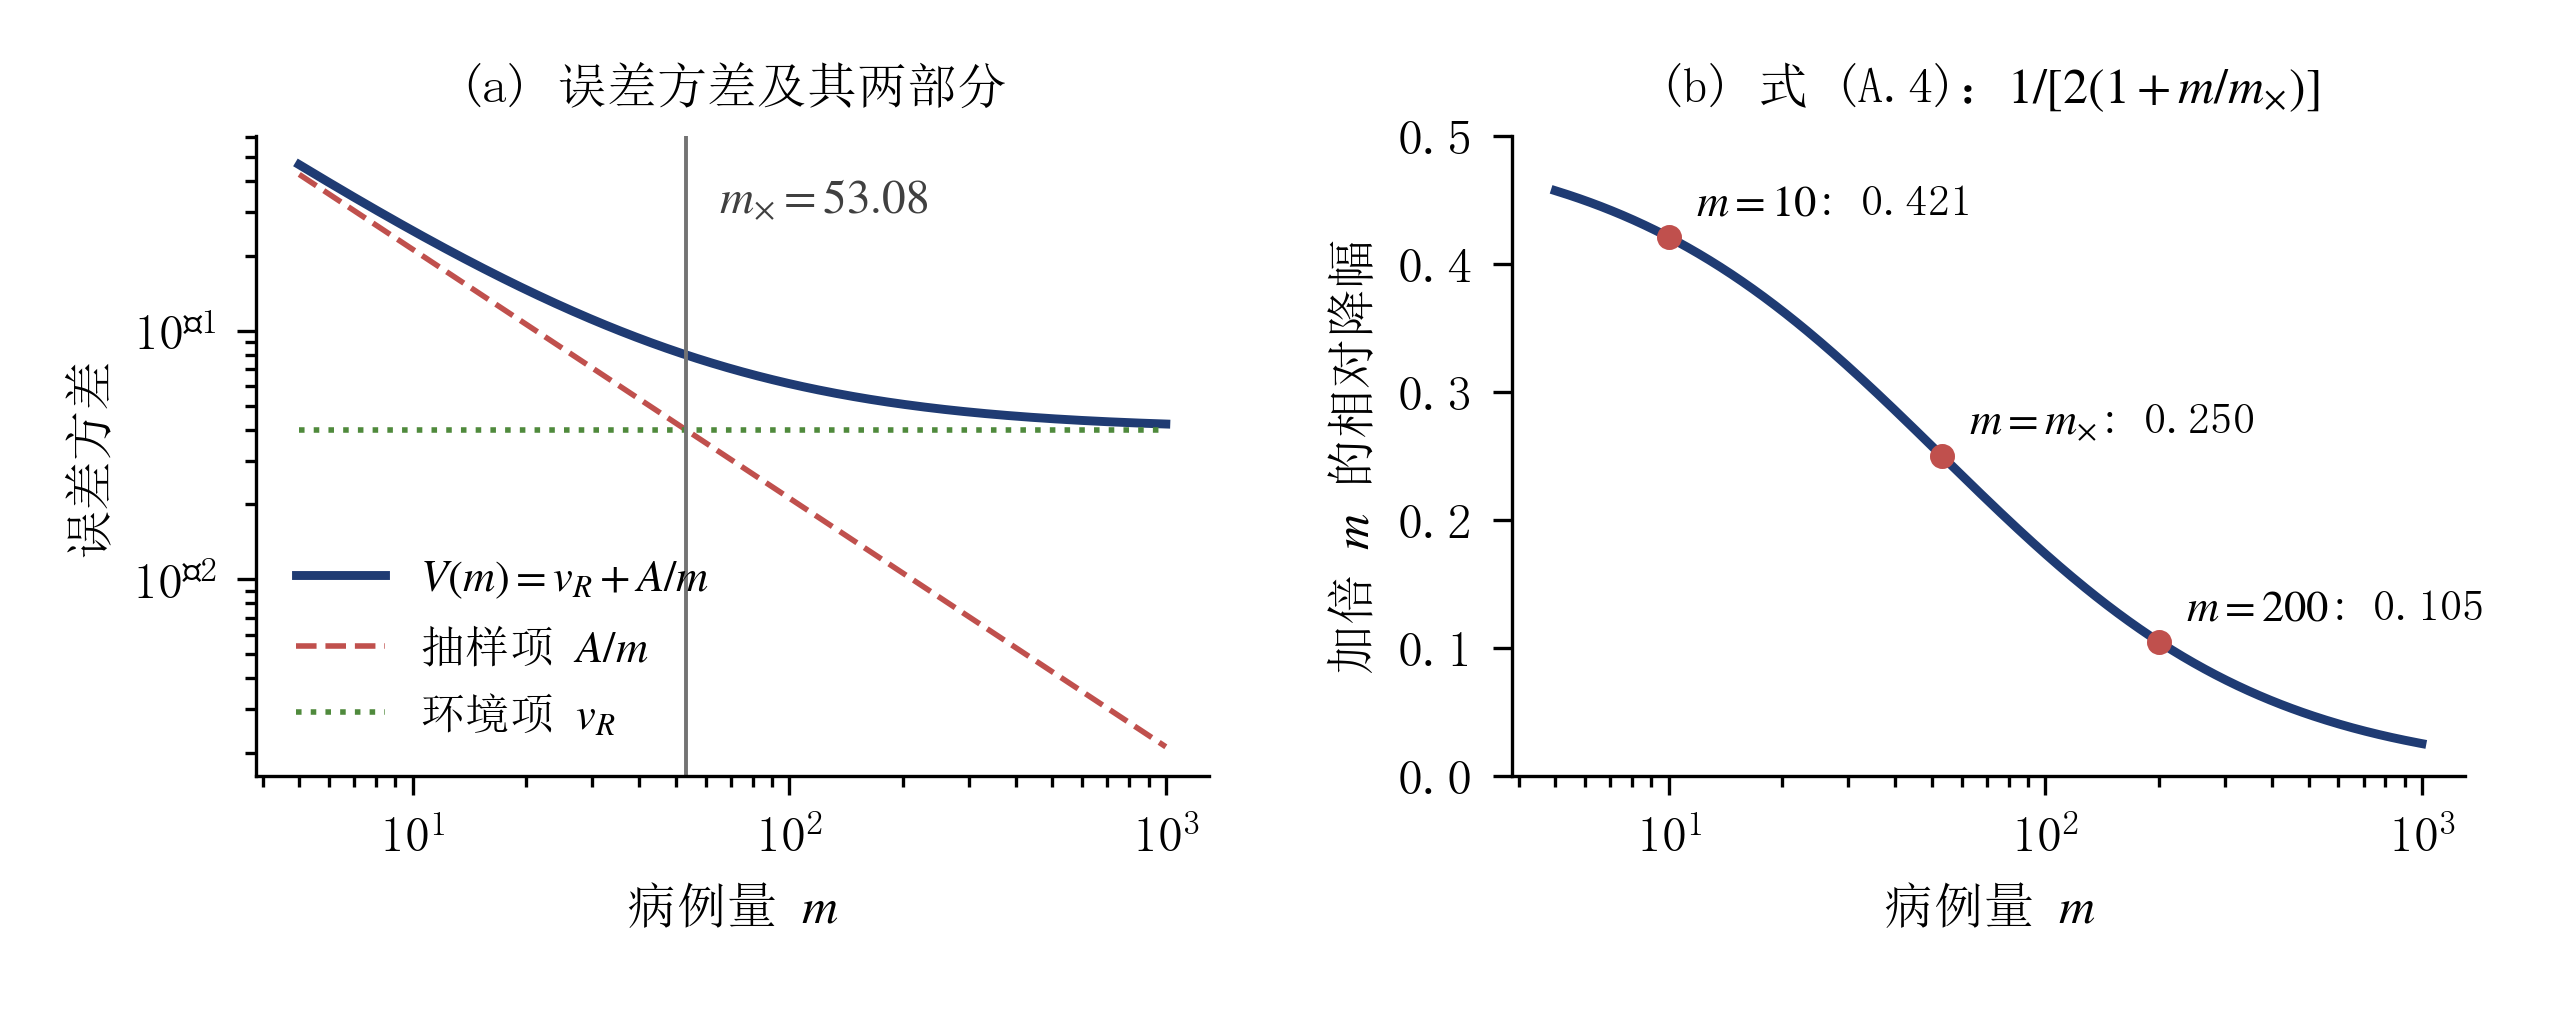
\includegraphics[width=\linewidth]{figures/fig-prop1.png}
\caption{命题 1 在基线参数式~\eqref{eq:baseline} 下的数值示意。(a) 误差方差 $V(m)=v_R+A/m$ 及其两部分，竖线为平衡规模 $\mx$；(b) 病例量加倍时的相对降幅，即式 (A.4)。}
\label{fig:prop1}
\end{figure}

固定 $n$ 而把 $\rho$ 加倍（要求 $2\rho\le1$）时，式 (4) 中只有报告项 $\Rbar/(\rho n)$ 减半，绝对降幅为 $\Rbar/(2\rho n)$，相对降幅为 $\Rbar/[2\rho nV(n,\rho)]$。取 $n=\mx/\rho=212.3$，此时 $V=2v_R=0.08$，相对降幅为
\begin{equation*}
\frac{1.15}{2\times53.08\times0.08}=0.1354 ,
\end{equation*}
低于沿 $n$ 路径加倍时的 $1/4$。

两条路径的对数边际由式 (4) 直接求导得到：
\begin{equation}
-\frac{\partial V}{\partial\log n}=\frac{\Rbar}{\rho n}+\frac{U}{kn}=\frac Am,\qquad
-\frac{\partial V}{\partial\log\rho}=\frac{\Rbar}{\rho n}=\frac{\Rbar}m .
\ptag{A.5}
\end{equation}
\zhu{$\partial/\partial\log n=n\,\partial/\partial n$，且 $n\,\partial(1/n)/\partial n=-1/n$；$\rho$ 只出现在报告项中。}
二者之比 $A/\Rbar$ 在基线下为 $2.1232/1.15=1.846$。式 (A.4) 只适用于固定 $\rho$ 的路径，$\rho$ 改变时 $A$ 随之改变。

\subsection{结论 (iv)：条件无偏估计的下界}

\begin{proof}[结论 (iv) 的证明]
\begin{enumerate}
\item 以 $R_t$ 为条件应用 (P6)：
\begin{equation*}
\E(\tilde\theta-\Rbar)^2=\E[\Var(\tilde\theta\mid R_t)]+\E\big[(\E(\tilde\theta\mid R_t)-\Rbar)^2\big]=\E[\Var(\tilde\theta\mid R_t)]+v_R .
\end{equation*}
\zhu{条件无偏使 $\E(\tilde\theta\mid R_t)=R_t$，第二项化为 $\Var R_t=v_R$。}
\item 对每个固定的 $R_t$，由 (P7) 与引理~\ref{lem:umvue}，$\Var(\tilde\theta\mid R_t)\ge1/\mathcal I(R_t)=R_t/(\rho n)+{R_t}^2/(kn)$。
\item 对 $R_t$ 取期望，$\E[1/\mathcal I(R_t)]+v_R=\Rbar/(\rho n)+U/(kn)+v_R=V$。取 $\tilde\theta=\Rhat_t$ 时第 2 步处处取等号（引理~\ref{lem:umvue}~第 6 步）。
\end{enumerate}
\end{proof}

同样的下界适用于一步预测。设 $R_{t+1}$ 与历史独立，$y=C_{t+1}/m$，$\hat y$ 为仅基于历史的预测，则
\begin{equation*}
\E(\hat y-y)^2=\E(\hat y-\E y)^2+\Var y\ \ge\ V .
\end{equation*}
\zhu{$\hat y$ 与 $y$ 独立，交叉项为零；$\Var y=V$ 由式 (4)；$\hat y=\Rbar$ 时取等号。}

\begin{conditions}
结论 (iv) 要求条件无偏对每个 $R_t$ 成立。向先验均值收缩的估计量不满足此条件，其均方误差可低于 $V$，见引理~\ref{lem:shrink}。
\end{conditions}

\subsection{自相关环境下的预测误差}

\begin{lemma}[论文第 2.2 节]\label{lem:ar1}
若 $R_t$ 为平稳 AR(1) 过程，方差 $v_R$，系数 $\phi$，则一步预测误差的环境部分为 $(1-\phi^2)v_R$。
\end{lemma}

\begin{yuan}
平稳 AR(1) 过程 $R_{t+1}-\Rbar=\phi(R_t-\Rbar)+e_{t+1}$，$e_t$ 为白噪声，自协方差 $\Cov(R_s,R_t)=v_R\phi^{\lvert s-t\rvert}$，见 \citet{hamilton1994time}。
\end{yuan}

\begin{proof}
最优线性预测为 $\Rbar+\phi(R_t-\Rbar)$，预测误差 $R_{t+1}-\Rbar-\phi(R_t-\Rbar)$ 的方差为
\begin{equation*}
v_R+\phi^2v_R-2\phi\Cov(R_{t+1},R_t)=v_R+\phi^2v_R-2\phi^2v_R=(1-\phi^2)v_R .
\end{equation*}
\zhu{$\Cov(R_{t+1},R_t)=\phi v_R$，取自协方差公式中 $\lvert s-t\rvert=1$。}
\end{proof}

\subsection{多辖区汇总}

\begin{lemma}[论文第 2.2 节，式 (5)]\label{lem:pool}
$J$ 个辖区的环境方差均为 $v_R$，$J(J-1)$ 个有序辖区对的相关系数平均为 $\bar c$，则辖区均值的环境方差为
\begin{equation}
\Var\Big(\frac1J\sum_{j=1}^JR_j\Big)=v_R\bar c+\frac{v_R(1-\bar c)}J .
\ptag{5}
\end{equation}
\end{lemma}

\begin{proof}
展开和的方差：
\begin{equation*}
\Var\Big(\frac1J\sum_jR_j\Big)=\frac1{J^2}\Big[\sum_j\Var R_j+\sum_{i\ne j}\Cov(R_i,R_j)\Big]=\frac{Jv_R+J(J-1)\bar cv_R}{J^2}=v_R\bar c+\frac{v_R(1-\bar c)}J .
\end{equation*}
\zhu{$\sum_{i\ne j}\Cov(R_i,R_j)=v_R\sum_{i\ne j}\Corr(R_i,R_j)=J(J-1)\bar cv_R$。}
\end{proof}

$J\to\infty$ 时式 (5) 趋于 $v_R\bar c$。辖区汇总只在 $\bar c<1$ 时降低环境方差。

\section{命题 2：报告异质性}\label{sec:prop2}

\begin{proposition}[论文第 2.3 节，式 (6)；附录 A.4]\label{prop:2}
在 H2--H5 下，
\begin{equation}
V_H(m)=v_R+v_H+\frac{A_H}m,\qquad v_H=\tau^2(\Rbar^2+v_R),\qquad A_H=\Rbar+\frac{\rho(1+\tau^2)(\Rbar^2+v_R)}{k} ,
\ptag{6}
\end{equation}
平衡规模 $m_{\times,H}=A_H/(v_R+v_H)<\mx$，且病例数的均值与方差只识别 $(1+\tau^2)(\Rbar^2+v_R)$。
\end{proposition}

\begin{yuan}
(P6)；引理~\ref{lem:cases}，以 $p_t$ 代替 $\rho$。
\end{yuan}

\begin{proof}
\begin{enumerate}
\item 给定 $(n,R_t,p_t)$，由引理~\ref{lem:cases}，$\E(C_t\mid n,R_t,p_t)=p_tnR_t$，$\Var(C_t\mid n,R_t,p_t)=p_tnR_t+{p_t}^2n{R_t}^2/k$。
\item 记 $\sigma^2=\Var p_t=\tau^2\rho^2$，则 $\E {p_t}^2=\rho^2+\sigma^2$。由 H5，$p_t$ 与 $(R_t,n)$ 独立，对 $p_t$ 应用 (P6)：
\begin{equation}
\Var(C_t\mid n,R_t)=\E\Big[p_tnR_t+\frac{{p_t}^2n{R_t}^2}{k}\Big]+\Var(p_tnR_t)=\rho nR_t+\frac{(\rho^2+\sigma^2)n{R_t}^2}{k}+\sigma^2n^2{R_t}^2 .
\ptag{A.6}
\end{equation}
\item 条件均值为 $\rho nR_t$，故 $\E(\Rhat_t\mid R_t)=R_t$，$\E\Rhat_t=\Rbar$。
\item 式 (A.6) 除以 $(\rho n)^2$，再对 $R_t$ 应用 (P6)：
\begin{equation}
V_H=\E\Big[\frac{R_t}{m}+\frac{(1+\tau^2)\rho {R_t}^2}{km}+\tau^2{R_t}^2\Big]+v_R
=v_R+\tau^2U+\frac{\Rbar}m+\frac{\rho(1+\tau^2)U}{km} .
\ptag{A.7}
\end{equation}
\zhu{逐项除以 $(\rho n)^2$：$\rho nR_t/(\rho n)^2=R_t/m$；$(\rho^2+\sigma^2)n{R_t}^2/[k(\rho n)^2]=(1+\tau^2){R_t}^2/(kn)=(1+\tau^2)\rho {R_t}^2/(km)$；$\sigma^2n^2{R_t}^2/(\rho n)^2=\tau^2{R_t}^2$。}
\item 记 $U_H=(1+\tau^2)U$，则 $v_R+v_H=U_H-\Rbar^2$，$A_H=\Rbar+\rho U_H/k$。均值 $\Rbar$ 与方差 $V_H$ 只通过 $U_H$ 依赖 $(v_R,\tau)$，两个矩不能把 $v_R$ 与 $\tau^2$ 分开。
\item 不等式 $A_H/(v_R+v_H)<A/v_R$ 两边乘正数 $v_R(v_R+v_H)$，等价于 $v_RA_H<A(v_R+v_H)$。代入 $A_H=A+\rho\tau^2U/k$ 与 $v_H=\tau^2U$，得 $v_R\rho\tau^2U/k<A\tau^2U$；$\tau>0$ 时它等价于 $\rho v_R/k<A$。而 $A-\rho v_R/k=\Rbar+\rho\Rbar^2/k>0$，故不等式成立。
\end{enumerate}
\end{proof}

代入基线值得
\begin{equation}\label{eq:mxH}
\begin{aligned}
&v_H=0.0225\times1.3625=0.0307,\qquad A_H=1.15+\frac{0.25\times1.0225\times1.3625}{0.35}=2.1451,\\
&m_{\times,H}=\frac{2.1451}{0.0707}=30.36 .
\end{aligned}
\end{equation}

\begin{conditions}
H2--H5。$\tau=0$ 时式 (6) 退回式 (4)。
\end{conditions}

\section{命题 3：固定预算的分配}\label{sec:prop3}

\begin{proposition}[论文第 2.3 节，式 (7)、(8)；附录 A.5]\label{prop:3}
固定 $\rho$，设 $R_t$ 各期独立。
\begin{enumerate}[label=(\roman*),leftmargin=2.2em]
\item $T$ 期均值的方差为
\begin{equation}
\Var\Big(\frac1T\sum_{t=1}^T\Rhat_t\Big)=\frac{v_R}T+\frac{A}{Tm} .
\ptag{7}
\end{equation}
\item 设 $c_0,c_1,v_R,A>0$，预算约束为 $\mathcal B=T(c_0+c_1m)$。若内点可行，式 (7) 的唯一最小点为
\begin{equation}
m^*=\sqrt{\frac{c_0}{c_1}\,\mx},\qquad T^*=\frac{\mathcal B}{c_0+c_1m^*}\ge1 .
\ptag{8}
\end{equation}
\end{enumerate}
\end{proposition}

\begin{yuan}
(P6)；式 (4)。两阶段抽样的最优单元内样本量 \citep{cochran1977sampling}：一级单元数 $n_1$，每单元抽 $m$ 个二级单元，成本 ${c_1}'n_1+{c_2}'n_1m$，方差 ${S_u}^2/n_1+{S_2}^2/(n_1m)$，最优 $m_{\mathrm{opt}}=(S_2/S_u)\sqrt{{c_1}'/{c_2}'}$。与本问题的对应为：一级单元对应时期，${S_u}^2$ 对应 $v_R$，${S_2}^2$ 对应 $A$，${c_1}'$ 对应 $c_0$，${c_2}'$ 对应 $c_1$。
\end{yuan}

\begin{proof}[式 (7) 的证明]
\begin{enumerate}
\item 以 $R_{1:T}=(R_1,\dots,R_T)$ 为条件应用 (P6)。给定 $R_{1:T}$，各期病例数独立，且 $\E(\Rhat_t\mid R_{1:T})=R_t$。
\item 条件方差部分为
\begin{equation*}
\E\Big[\Var\Big(\frac1T\sum_t\Rhat_t\,\Big|\,R_{1:T}\Big)\Big]=\frac1{T^2}\sum_t\E\Big[\frac{R_t}m+\frac{\rho {R_t}^2}{km}\Big]=\frac1{T^2}\cdot T\cdot\frac Am=\frac A{Tm} .
\end{equation*}
\zhu{用式~\eqref{eq:condvar}，$\E R_t=\Rbar$，$\E {R_t}^2=U$。}
\item 条件均值部分为 $\Var\bar R_T$，$\bar R_T=T^{-1}\sum_tR_t$；各期独立时等于 $v_R/T$。两部分相加即式 (7)，即论文式 (A.8)。
\end{enumerate}
\end{proof}

\begin{proof}[式 (8) 的证明]
\begin{enumerate}
\item 由预算约束，$T=\mathcal B/(c_0+c_1m)$。代入式 (7)，目标函数为
\begin{equation*}
f(m)=\frac1T\Big(v_R+\frac Am\Big)=\frac{(c_0+c_1m)(v_R+A/m)}{\mathcal B} .
\end{equation*}
\item 展开得 $\mathcal Bf(m)=c_0v_R+c_0A/m+c_1v_Rm+c_1A$。
\item 求导得 $\mathcal Bf'(m)=c_1v_R-c_0A/m^2$，$\mathcal Bf''(m)=2c_0A/m^3>0$，故 $f$ 在 $m>0$ 上严格凸。
\item 令 $f'(m)=0$，得 $m^{*2}=c_0A/(c_1v_R)=(c_0/c_1)\mx$。严格凸函数的驻点唯一，且为全局最小点。这一步即论文式 (A.9)。
\end{enumerate}
\end{proof}

代入式~\eqref{eq:mx}，$c_0/c_1=10$ 时 $m^*=\sqrt{530.8}=23.04$，$c_0/c_1=100$ 时 $m^*=72.86$。若平衡规模取第~\ref{sec:observed}~节的潜在值 $21.3$--$49.2$，则 $m^*$ 在 $c_0/c_1=10$ 时为 $14.6$--$22.2$，在 $c_0/c_1=100$ 时为 $46.1$--$70.1$。

\begin{conditions}
固定 $\rho$，$R_t$ 各期独立；自相关情形见引理~\ref{lem:C2}。$v_R=0$ 时 $\mathcal Bf'=-c_0A/m^2<0$ 恒成立，$f$ 随 $m$ 单调下降，不存在有限内点解。$T$ 须为不小于 1 的整数且 $m$ 有上限时，还须把内点解与边界解比较。
\end{conditions}

\subsection{自相关环境下的相关和}

\begin{lemma}[论文第 2.3 节，式 (9)]\label{lem:S}
若 $\Cov(R_s,R_t)=v_R\phi^{\lvert s-t\rvert}$，$\phi\ne1$，则 $T^2\Var\bar R_T=v_RS(\phi,T)$，其中
\begin{equation}
S(\phi,T)=\sum_{s,t=1}^{T}\phi^{\lvert s-t\rvert}=\frac{T(1+\phi)}{1-\phi}-\frac{2\phi(1-\phi^T)}{(1-\phi)^2} .
\ptag{9}
\end{equation}
\end{lemma}

\begin{yuan}
AR(1) 自协方差（引理~\ref{lem:ar1}）；有限几何级数 $\sum_{h=1}^{j}\phi^h=\phi(1-\phi^j)/(1-\phi)$。
\end{yuan}

\begin{proof}
\begin{enumerate}
\item 按滞后 $h=\lvert s-t\rvert$ 归并：
\begin{equation*}
T^2\Var\bar R_T=\sum_{s,t}\Cov(R_s,R_t)=v_R\Big[T+2\sum_{h=1}^{T-1}(T-h)\phi^h\Big].
\end{equation*}
\zhu{滞后为 $h\ge1$ 且 $s<t$ 的有序对共 $T-h$ 个，$s>t$ 的同样多，故系数为 2。}
\item 交换求和次序：$\sum_{h=1}^{T-1}(T-h)\phi^h=\sum_{j=1}^{T-1}\sum_{h=1}^{j}\phi^h$。
\zhu{对固定的 $h$，满足 $h\le j\le T-1$ 的 $j$ 恰有 $T-h$ 个。}
\item 内层用有限几何级数：
\begin{equation*}
\sum_{j=1}^{T-1}\frac{\phi(1-\phi^j)}{1-\phi}=\frac{\phi(T-1)}{1-\phi}-\frac{\phi^2(1-\phi^{T-1})}{(1-\phi)^2} .
\end{equation*}
\item 通分整理：
\begin{equation*}
\frac{\phi(T-1)(1-\phi)-\phi^2+\phi^{T+1}}{(1-\phi)^2}=\frac{T\phi(1-\phi)-\phi(1-\phi^T)}{(1-\phi)^2} .
\end{equation*}
\zhu{两边分子展开后均为 $T\phi-T\phi^2-\phi+\phi^{T+1}$。}
\item 代回第 1 步：
\begin{equation*}
S=T+\frac{2T\phi}{1-\phi}-\frac{2\phi(1-\phi^T)}{(1-\phi)^2}=\frac{T(1+\phi)}{1-\phi}-\frac{2\phi(1-\phi^T)}{(1-\phi)^2} .
\end{equation*}
\end{enumerate}
\end{proof}

式 (9) 满足 $S(\phi,1)=1$，$S(\phi,2)=2+2\phi$，且 $\phi\to0$ 时 $S\to T$。表 S7 脚注把它写作 $S=\sum_{\lvert h\rvert<T}(T-\lvert h\rvert)\phi^{\lvert h\rvert}$，与第 1 步相同。数值上，
\begin{equation}\label{eq:Svals}
S(0.5,10)=30-3.9961=26.0039,\qquad S(0.25,10)=15.7778 .
\end{equation}
于是在 AR(1) 环境下，式 (7) 的环境项 $v_R/T$ 换成 $v_RS(\phi,T)/T^2$。

\subsection{固定覆盖规模时的报告概率}

\begin{lemma}[论文附录 A.5，式 (A.10)]\label{lem:rho}
固定 $n$，令 $H=v_R+U/(kn)$，$Q=\Rbar/n$，单期成本为 $c_0+c_\rho\rho$。内点最优报告概率为
\begin{equation}
\rho^*=\sqrt{\frac{c_0Q}{c_\rho H}} ,
\ptag{A.10}
\end{equation}
超出 $(0,1]$ 时截取到端点。若成本按 $c_0+c_1m$ 计价，则 $c_\rho=c_1n$。
\end{lemma}

\begin{proof}
\begin{enumerate}
\item 固定 $n$ 时式 (4) 写成 $V=H+Q/\rho$。由 $T=\mathcal B/c(\rho)$，目标为 $f(\rho)=c(\rho)(H+Q/\rho)/\mathcal B$。
\item 代入 $c(\rho)=c_0+c_\rho\rho$ 并展开：$\mathcal Bf=c_0H+c_0Q/\rho+c_\rho H\rho+c_\rho Q$。
\item 求导：$\mathcal Bf'=-c_0Q/\rho^2+c_\rho H$，$\mathcal Bf''=2c_0Q/\rho^3>0$。令 $f'=0$ 得 $\rho^{*2}=c_0Q/(c_\rho H)$，严格凸保证它是唯一最小点。
\item $c_0+c_1m=c_0+c_1n\rho$，故 $c_\rho=c_1n$。
\end{enumerate}
\end{proof}

取 $n=212.3$，$c_0=100$，$c_1=1$，代入基线值得 $H=0.04+1.3625/(0.35\times212.3)=0.05834$，$Q=0.005416$，
\begin{equation}\label{eq:rhostar}
\rho^*=\sqrt{\frac{100\times0.005416}{212.3\times0.05834}}=0.2091 .
\end{equation}

\subsection{表 S7 的三项分解}

表 S7 与结果第 3.1 节在 AR(1) 环境之外还允许报告波动自相关。论文给出了下式的数值，未写出推导；下面补全，记号 $\psi$ 的定义见第~\ref{sec:errata}~节 E8。

\begin{lemma}[表 S7；结果第 3.1 节]\label{lem:s7}
设 $R_t$ 为 AR(1) 过程（系数 $\phi$，方差 $v_R$）；报告波动 $\varepsilon_t=p_t/\rho-1$ 为与 $R$ 过程独立的平稳过程，$\E\varepsilon_t=0$，$\Var\varepsilon_t=\tau^2$，$\Corr(\varepsilon_s,\varepsilon_t)=\psi^{\lvert s-t\rvert}$；其余同命题~\ref{prop:2}。则 $T$ 期均值的均方误差为
\begin{equation}\label{eq:s7}
\frac{v_RS(\phi,T)}{T^2}
+\frac{\tau^2\big[\Rbar^2S(\psi,T)+v_RS(\phi\psi,T)\big]}{T^2}
+\frac{A_H}{Tm} ,
\end{equation}
三项依次为环境项、报告项与抽样项。
\end{lemma}

\begin{proof}
\begin{enumerate}
\item 以 $(R_{1:T},p_{1:T})$ 为条件应用 (P6)。条件均值为 $\E(\Rhat_t\mid R_{1:T},p_{1:T})=(p_t/\rho)R_t=(1+\varepsilon_t)R_t$。
\item 条件方差部分为
\begin{equation*}
\E\Var(\Rhat_t\mid\cdot)=\E\Big[\frac{p_tR_t}{\rho m}+\frac{{p_t}^2{R_t}^2}{k\rho^2n}\Big]=\frac{\Rbar}m+\frac{\rho(1+\tau^2)U}{km}=\frac{A_H}m .
\end{equation*}
\zhu{与命题~\ref{prop:2}~证明第 4 步相同。给定条件时各期独立，$T$ 期平均后为 $A_H/(Tm)$。}
\item 条件均值部分展开为
\begin{equation*}
\Var\Big(\frac1T\sum_tR_t(1+\varepsilon_t)\Big)=\frac1{T^2}\Big[\Var\sum_tR_t+\Var\sum_t\varepsilon_tR_t+2\Cov\Big(\sum_sR_s,\sum_t\varepsilon_tR_t\Big)\Big].
\end{equation*}
\item 交叉项为零：$\Cov(R_s,\varepsilon_tR_t)=\E[\varepsilon_t]\,\E[(R_s-\Rbar)R_t]=0$。
\zhu{$\varepsilon$ 过程与 $R$ 过程独立，且 $\E\varepsilon_t=0$。}
\item 报告项为
\begin{equation*}
\Var\sum_t\varepsilon_tR_t=\sum_{s,t}\E[\varepsilon_s\varepsilon_t]\,\E[R_sR_t]=\sum_{s,t}\tau^2\psi^{\lvert s-t\rvert}\big(\Rbar^2+v_R\phi^{\lvert s-t\rvert}\big)=\tau^2\big[\Rbar^2S(\psi,T)+v_RS(\phi\psi,T)\big].
\end{equation*}
\zhu{$\E\sum\varepsilon_tR_t=0$，故方差等于二阶矩；独立性使期望分解；$\E R_sR_t=\Rbar^2+\Cov(R_s,R_t)$；最后用式 (9) 的求和形式。}
\item 环境项为 $\Var\sum_tR_t=v_RS(\phi,T)$（引理~\ref{lem:S}）。三部分相加即式~\eqref{eq:s7}。
\end{enumerate}
\end{proof}

取 $T=10$，$m=50$，$\phi=\psi=0.5$，$\tau=0.15$，并用式~\eqref{eq:Svals}，三项依次为
\begin{equation*}
\begin{aligned}
&\frac{0.04\times26.0039}{100}=10.40\times10^{-3},\\
&\frac{0.0225\times(1.3225\times26.0039+0.04\times15.7778)}{100}=7.88\times10^{-3},\qquad
\frac{2.1451}{500}=4.29\times10^{-3},
\end{aligned}
\end{equation*}
合计 $22.57\times10^{-3}$。在同一设定下改变一个量：病例量增至 500 时为 $18.71\times10^{-3}$；$\tau=0$ 时为 $14.65\times10^{-3}$；$T=40$ 时为 $6.17\times10^{-3}$；预算加倍全部用于病例（$m=200$）时为 $19.35\times10^{-3}$，全部用于时期（$T=20$）时为 $11.98\times10^{-3}$。

\section{推论 1：覆盖规模与报告完整度}\label{sec:cor1}

\begin{corollary}[论文第 2.3 节，式 (10)；附录 A.6]\label{cor:1}
记 $U_0=\Rbar^2+v_R$。
\begin{enumerate}[label=(\roman*),leftmargin=2.2em]
\item 若 $\tau$ 不依赖 $\rho$，按相同比例扩大 $n$ 比提高 $\rho$ 使 $V_H$ 下降更多。
\item 若 $\Var(p_t)=\rho(1-\rho)/(\nu+1)$，则当且仅当
\begin{equation}
m>\frac{\rho^2\nu}{k}
\ptag{10}
\end{equation}
时提高 $\rho$ 的对数边际大于扩大 $n$ 的对数边际。
\end{enumerate}
\end{corollary}

\begin{yuan}
式 (6)；$\partial/\partial\log x=x\,\partial/\partial x$。
\end{yuan}

\begin{proof}
\begin{enumerate}
\item 用 $n$、$\rho$ 写出式 (6)：
\begin{equation*}
V_H=v_R+\tau^2U_0+\frac{\Rbar}{\rho n}+\frac{(1+\tau^2)U_0}{kn} .
\end{equation*}
\zhu{$A_H/m$ 中的 $\rho/m=1/n$。}
\item 对 $\log n$ 求导（$\tau$ 与 $n$ 无关）：$-\partial V_H/\partial\log n=\Rbar/(\rho n)+(1+\tau^2)U_0/(kn)$。
\item 对 $\log\rho$ 求导，允许 $\tau^2$ 依赖 $\rho$：
\begin{equation}
-\frac{\partial V_H}{\partial\log\rho}=\frac{\Rbar}{\rho n}-\rho\,\frac{\mathrm d\tau^2}{\mathrm d\rho}\,U_0\Big(1+\frac1{kn}\Big).
\ptag{A.11}
\end{equation}
\zhu{$\tau^2$ 出现在 $\tau^2U_0$ 与 $\tau^2U_0/(kn)$ 两处。}
\item 若 $\mathrm d\tau^2/\mathrm d\rho=0$，第 2 步减第 3 步得 $(1+\tau^2)U_0/(kn)>0$，结论 (i) 成立。
\item 若 $\Var p_t=\rho(1-\rho)/(\nu+1)$，则 $\tau^2=\Var p_t/\rho^2=\dfrac{1-\rho}{\rho(\nu+1)}$，$\rho\dfrac{\mathrm d\tau^2}{\mathrm d\rho}=-\dfrac1{\rho(\nu+1)}$。
\item 第 3 步减第 2 步：
\begin{equation}
\frac{U_0}{\rho(\nu+1)}\Big(1+\frac1{kn}\Big)-\frac{(1+\tau^2)U_0}{kn}
=\frac{U_0}{kn}\Big[\frac{kn+1}{\rho(\nu+1)}-1-\frac{1-\rho}{\rho(\nu+1)}\Big]
=\frac{U_0}{kn}\Big[\frac{kn+\rho}{\rho(\nu+1)}-1\Big].
\ptag{A.12}
\end{equation}
\zhu{代入第 5 步的 $\tau^2$，并把前两项通分到 $kn$。}
\item 方括号为正当且仅当 $kn+\rho>\rho\nu+\rho$，即 $kn>\rho\nu$，亦即 $m=\rho n>\rho^2\nu/k$。
\end{enumerate}
\end{proof}

\begin{conditions}
论文称 $\Var(p_t)=\rho(1-\rho)/(\nu+1)$ 来自“对 $\nu$ 个单位的二项抽样”。若 $p_t=\Bin(\nu,\rho)/\nu$，方差为 $\rho(1-\rho)/\nu$；分母 $\nu+1$ 对应 $p_t\sim\mathrm{Beta}(\rho\nu,(1-\rho)\nu)$。按二项方差重做第 5--7 步，$\tau^2=(1-\rho)/(\rho\nu)$，$\rho\,\mathrm d\tau^2/\mathrm d\rho=-1/(\rho\nu)$，两边际之差为 $\dfrac{U_0}{kn}\Big[\dfrac{kn+\rho}{\rho\nu}-1\Big]$，切换条件变为
\begin{equation}\label{eq:cor1bin}
m>\frac{\rho^2(\nu-1)}{k} .
\end{equation}
两个阈值相差 $\rho^2/k$，基线下约为 $0.18$ 例，结论方向不变（第~\ref{sec:errata}~节 E1）。
\end{conditions}

\section{观测统计量与随机分母}\label{sec:observed}

第~\ref{sec:model}--\ref{sec:cor1}~节的分母 $n$ 由设计固定。论文第 2.5--2.6 节转向实证数据，分母换成由过去报告数构成的感染压力代理，本节推导由此产生的附加项。

\subsection{加权增长比}

\begin{definition}[论文第 2.5 节，式 (11)]\label{def:G}
加权增长比定义为
\begin{equation}
G_t=\frac{C_{t+1}}{D_t},\qquad D_t=0.65\,C_t+0.25\,C_{t-1}+0.10\,C_{t-2} .
\ptag{11}
\end{equation}
权重 $w=(0.65,0.25,0.10)$ 满足 $\sum_jw_j=1$，$\sum_j{w_j}^2=0.4225+0.0625+0.01=0.495$。
\end{definition}

$D_t$ 是更新方程中感染压力 $\Lambda_{t+1}=\sum_jw_jI_{t+1-j}$ 的观测代理。\citet[式 (7)]{fraser2007estimating} 给出 $R(t)=I(t)\big/\int_{\,(0,\infty)} I(t-\tau)w(\tau)\,\mathrm d\tau$；$G_t$ 是它以周为步长、以报告数代替感染数的离散形式。

\subsection{更新型比值}

\begin{lemma}[论文第 2.5 节，式 (12)]\label{lem:RA}
代际间隔取伽马分布，均值 $3.6$ 天，标准差 $1.6$ 天，则
\begin{equation}
R_{A,t}=(1+r_t\theta)^{\alpha},\qquad r_t=\frac17\log\frac{C_{t+1}+0.5}{C_t+0.5},
\ptag{12}
\end{equation}
其中形状 $\alpha=(3.6/1.6)^2=5.0625$，尺度 $\theta=1.6^2/3.6=0.7111$ 天。
\end{lemma}

\begin{yuan}
\citet[Sec.~2(b)，式 (2.8)、(2.9)]{wallinga2007how}：增长率 $r$ 与再生数 $R$ 的关系为
\begin{equation*}
M(z)=\int_{\,(0,\infty)} e^{za}g(a)\,\mathrm da,\qquad R=\frac1{M(-r)},
\end{equation*}
$g$ 为代际间隔密度，$M$ 为其矩母函数。原文第 3 节给出指数分布（式 (3.1)）与多阶段分布（式 (3.3)）两个特例，未写伽马形式。序列间隔均值 $3.6$ 天（95\% 置信区间 $2.9$--$4.3$）、标准差 $1.6$ 天取自 \citet[摘要 Results]{cowling2009estimation}。伽马矩母函数 (P12)。
\end{yuan}

\begin{proof}
\begin{enumerate}
\item 在 (P12) 中取 $z=-r$，得 $M(-r)=(1+r\theta)^{-\alpha}$，要求 $1+r\theta>0$。
\item 代入 Wallinga--Lipsitch 式 (2.9)，$R=1/M(-r)=(1+r\theta)^{\alpha}$。
\item 伽马矩匹配：$\alpha\theta=3.6$，$\alpha\theta^2=1.6^2$。两式相除得 $\theta=1.6^2/3.6=0.7111$，再由 $\alpha=3.6/\theta$ 得 $\alpha=(3.6/1.6)^2=5.0625$。
\item 指数增长下 $C_{t+1}=C_te^{7r}$，故日增长率 $r=\frac17\log(C_{t+1}/C_t)$。分子分母各加 $0.5$ 是连续性校正，使零计数时比值有定义。
\end{enumerate}
\end{proof}

\begin{conditions}
增长率 $r$ 在一周内恒定，且 $1+r\theta>0$。$R_A$ 是由观测增长率变换得到的表观量，其抽样性质见引理~\ref{lem:B6}。
\end{conditions}

\subsection{更新方程下的预测方差}

\begin{lemma}[论文第 2.5 节，式 (13)；附录 A.7，式 (A.13)]\label{lem:eq13}
令 $\bar\Lambda=\E(\Lambda_{t+1}\mid\mathcal F_t)$，$m=\rho\bar\Lambda$，$\CV(\Lambda_{t+1}\mid\mathcal F_t)$ 为感染压力的条件变异系数。在下列前提 (a)(b) 下，
\begin{equation}
\frac{\Var(C_{t+1}\mid\mathcal F_t)}{m^2}=v_R+\frac Am+\CV^2(\Lambda_{t+1}\mid\mathcal F_t)\,(\Rbar^2+v_R) .
\ptag{13}
\end{equation}
\begin{enumerate}[label=(\alph*),leftmargin=2.2em]
\item 给定 $(\Lambda_{t+1},R_{t+1})$，$I_{t+1}\sim\NB\big(k\Lambda_{t+1},k/(k+R_{t+1})\big)$，即每单位感染压力的后代按式 (1) 产生且可加；
\item 给定 $\mathcal F_t$，$\Lambda_{t+1}$ 与 $R_{t+1}$ 独立，$\E(R_{t+1}\mid\mathcal F_t)=\Rbar$，$\Var(R_{t+1}\mid\mathcal F_t)=v_R$。
\end{enumerate}
\end{lemma}

\begin{yuan}
更新方程 $\E(I_{t+1}\mid\Lambda_{t+1},R_{t+1})=R_{t+1}\Lambda_{t+1}$，见 \citet[Materials and Methods 第 3 段]{cori2013new} 与 \citet[式 (6)]{fraser2007estimating}；(P3)、(P4)、(P6)。前提 (a)(b) 为论文未写明的条件，见第~\ref{sec:errata}~节 E6。
\end{yuan}

\begin{proof}
以下省略下标 $t+1$。
\begin{enumerate}
\item 由 (a) 与 (P4)，$C\mid\Lambda,R\sim\NB(k\Lambda,k/(k+\rho R))$，条件均值 $\rho\Lambda R$，条件方差 $\rho\Lambda R+\rho^2\Lambda R^2/k$。
\zhu{与引理~\ref{lem:cases}~的证明相同，只是把 $n$ 换成 $\Lambda$。}
\item 条件方差的期望：由 (b)，
\begin{equation*}
\E\Big[\rho\Lambda R+\frac{\rho^2\Lambda R^2}{k}\,\Big|\,\mathcal F_t\Big]=\rho\bar\Lambda\Rbar+\frac{\rho^2\bar\Lambda U}{k}=m\Big(\Rbar+\frac{\rho U}{k}\Big)=mA .
\end{equation*}
\item 条件均值的方差：
\begin{equation*}
\Var(\rho\Lambda R\mid\mathcal F_t)=\rho^2\big[\E\Lambda^2\,\E R^2-\bar\Lambda^2\Rbar^2\big]=\rho^2\bar\Lambda^2\big[(1+\CV^2)U-\Rbar^2\big]=\rho^2\bar\Lambda^2\big[v_R+\CV^2U\big].
\end{equation*}
\zhu{$\E\Lambda^2=\bar\Lambda^2(1+\CV^2)$；(b) 的独立性使 $\E(\Lambda^2R^2)=\E\Lambda^2\,\E R^2$；$U-\Rbar^2=v_R$。}
\item 由 (P6) 把第 2、3 步相加，再除以 $m^2=\rho^2\bar\Lambda^2$，即得式 (13)。
\end{enumerate}
\end{proof}

与式 (4) 相比，式 (13) 多出 $\CV^2U$。这一项来自感染压力本身的不确定性，与规模 $m$ 无关。

\subsection{仿射损失模型与潜在平衡规模}

\begin{lemma}[论文第 2.6 节，式 (14)；附录 B.2]\label{lem:affine}
相对损失 $L_t=[(X_t-\bar X)/\bar X]^2$ 的仿射模型为
\begin{equation}
\E(L_t\mid M_t)=a+\frac b{M_t} .
\ptag{14}
\end{equation}
在理想情形下（一代恰为一周，无报告延迟，$\rho$ 已知，分母无噪声），$a=v_R/\Rbar^2$，$b=A/\Rbar^2$，$b/a=\mx$。$a,b>0$ 时局部对数斜率为
\begin{equation}\label{eq:slope}
\frac{\mathrm d\log(a+b/M)}{\mathrm d\log M}=-\frac1{1+M/(b/a)}\in(-1,0) .
\end{equation}
\end{lemma}

\begin{proof}
\begin{enumerate}
\item 理想情形下 $X_t=\Rhat_t$，$M_t=m$，中心取真值 $\bar X=\Rbar$。
\item 由式 (4)，$\E L_t=\E(\Rhat_t-\Rbar)^2/\Rbar^2=V/\Rbar^2=v_R/\Rbar^2+A/(\Rbar^2m)$。
\item 与 $a+b/m$ 逐项对照，$a=v_R/\Rbar^2$，$b=A/\Rbar^2$，$b/a=A/v_R=\mx$。
\item 求对数导数：
\begin{equation*}
\frac{\mathrm d\log(a+b/M)}{\mathrm d\log M}=\frac{-b/M}{a+b/M}=-\frac{b}{aM+b}=-\frac1{1+M/(b/a)} .
\end{equation*}
\zhu{$\mathrm d(b/M)/\mathrm d\log M=-b/M$。斜率在 $M=b/a$ 处为 $-1/2$。}
\end{enumerate}
\end{proof}

\begin{conditions}
中心取样本均值时，$\E L_t$ 有 $O(1/N)$ 偏差，$N$ 为样本量。一般的更新与延迟模型下，$b/a$ 与 $\mx$ 不恒等，二者的对应需要按论文第 2.11 节的模拟校准建立。附录 B.2 把 $m=\rho\Lambda$ 解释为报告后的有效感染压力，它与当期病例数没有恒等关系，$D_t$ 与 $C_t$ 都只是代理；理想模型中取 $n=\Lambda$，即回到第~\ref{sec:model}--\ref{sec:prop1}~节的固定分母结果。
\end{conditions}

论文第 2.6 节的潜在平衡规模情景取 $G$ 的样本均值 $\Rbar=1.6706$，$v_R\in\{0.04,0.08\}$，$k\in\{0.2,0.5\}$，$\rho\in\{0.0056,0.021\}$。$\rho$ 很小，故 $A\approx\Rbar$。按 $\mx=A/v_R$ 计算，范围的两端为
\begin{equation}\label{eq:latent}
\frac{1.6706+0.0056\times2.8709/0.5}{0.08}=21.28,\qquad
\frac{1.6706+0.021\times2.8309/0.2}{0.04}=49.20 ,
\end{equation}
其中 $2.8709=1.6706^2+0.08$，$2.8309=1.6706^2+0.04$。$k$ 与 $\rho$ 取值的出处见第~\ref{sec:errata}~节 E5、E7。

\subsection{分母二项噪声}

\begin{lemma}[论文第 2.6 节，式 (15)；附录 A.7，式 (A.14)]\label{lem:eq15}
设分母只含二项噪声，相对方差为 $c_w/m$，$c_w=(1-\rho)\sum_j{w_j}^2$，且分母噪声与分子独立，则
\begin{equation}
b\approx\frac{A+(1-\rho)(\Rbar^2+v_R)\sum_j{w_j}^2}{\Rbar^2} .
\ptag{15}
\end{equation}
相对方差 $c_w/m$ 成立需要以下前提：
\begin{enumerate}[label=(\alph*),leftmargin=2.2em,start=3]
\item 给定潜在计数 $Z$，各滞后报告数 $C_{t-j}\sim\Bin(Z_{t-j},\rho)$ 相互独立；
\item 各滞后潜在计数相等，即平坦路径 $Z_{t-j}\equiv Z$；
\item $\sum_jw_j=1$。
\end{enumerate}
\end{lemma}

\begin{yuan}
二项方差 $\Var\Bin(Z,\rho)=Z\rho(1-\rho)$；$(1+\delta)^{-1}$ 的 Taylor 展开；式 (4)。前提 (c)--(e) 为论文未写明的条件，见第~\ref{sec:errata}~节 E6。
\end{yuan}

\begin{proof}
\begin{enumerate}
\item 先求 $c_w$。在 (c)--(e) 下，$\E D_t=\rho Z\sum_jw_j=\rho Z=:m$，$\Var D_t=\sum_j{w_j}^2Z\rho(1-\rho)$，故 $\Var(D_t/m)=(1-\rho)\sum_j{w_j}^2/m=c_w/m$。
\item 记 $D_t=m(1+\delta)$，$Y=C_{t+1}/m$，则 $G=Y/(1+\delta)$。$Y$ 与 $\delta$ 独立，$\E Y=\Rbar$，$\Var Y=v_R+A/m$，$\E\delta=0$，$\E\delta^2=c_w/m$。
\item 二阶展开：$(1+\delta)^{-1}=1-\delta+\delta^2+O(\delta^3)$，$(1+\delta)^{-2}=1-2\delta+3\delta^2+O(\delta^3)$。
\item $\E G=\E Y\cdot\E(1+\delta)^{-1}=\Rbar(1+c_w/m)+O(m^{-2})$。
\zhu{独立性使期望相乘；二项噪声的 $\E\delta^3=O(m^{-2})$。}
\item $\E G^2=\E Y^2\cdot\E(1+\delta)^{-2}=(U+A/m)(1+3c_w/m)+O(m^{-2})$。
\zhu{$\E Y^2=\Rbar^2+\Var Y=U+A/m$。}
\item 由第 4、5 步，
\begin{equation*}
\Var G=(U+A/m)(1+3c_w/m)-\Rbar^2(1+2c_w/m)+O(m^{-2})=v_R+\frac{A+(\Rbar^2+3v_R)c_w}{m}+O(m^{-2}) .
\end{equation*}
\zhu{$3U-2\Rbar^2=\Rbar^2+3v_R$。}
\item 除以 $(\E G)^2=\Rbar^2(1+2c_w/m)+O(m^{-2})$，即乘以 $\Rbar^{-2}(1-2c_w/m)$：
\begin{equation}
\begin{aligned}
\frac{\Var G}{(\E G)^2}&=\frac{v_R}{\Rbar^2}+\frac{A+(\Rbar^2+3v_R)c_w-2v_Rc_w}{\Rbar^2m}+O(m^{-2})\\
&=\frac{v_R}{\Rbar^2}+\frac{A+(\Rbar^2+v_R)c_w}{\Rbar^2m}+O(m^{-2}) .
\end{aligned}
\ptag{A.14}
\end{equation}
\item 与 $a+b/m$ 对照即得式 (15)：截距不变，斜率增加 $(\Rbar^2+v_R)c_w/\Rbar^2$。
\end{enumerate}
\end{proof}

代入式 (11) 的权重，$c_w=0.495(1-\rho)$。分子与分母共享报告冲击时，独立性不成立，见第~\ref{sec:shock}~节。

\subsection{分子与分母共享的报告冲击}\label{sec:shock}

附录 B.1 允许报告冲击同时进入分子与分母。条件于无报告扰动的正计数路径 $Z$，设
\begin{equation}
C_t=\rho Z_t(1+\varepsilon_t),\qquad \E(\varepsilon_t\mid Z)=0,\qquad K(t,s)=\Cov(\varepsilon_t,\varepsilon_s\mid Z) ,
\ptag{B.1}
\end{equation}
并记
\begin{equation*}
\Lambda_t=\sum_{j\ge1}w_jZ_{t-j},\qquad q_{tj}=\frac{w_jZ_{t-j}}{\Lambda_t},\qquad u_t=\sum_jq_{tj}\varepsilon_{t-j},\qquad y_t=\frac{Z_t}{\Lambda_t},\qquad Y_t=y_t\,\frac{1+\varepsilon_t}{1+u_t} .
\end{equation*}
分母为 $\sum_jw_jC_{t-j}=\rho\sum_jw_jZ_{t-j}(1+\varepsilon_{t-j})=\rho\Lambda_t(1+u_t)$，$\rho$ 在比值中约去，故 $Y_t$ 是观测比值。路径权重满足 $\sum_jq_{tj}=1$，只在平坦路径上 $q_{tj}=w_j$。记 $q_t=(q_{t1},q_{t2},\dots)^\top$，$K_{--}$ 为滞后冲击 $(\varepsilon_{t-1},\varepsilon_{t-2},\dots)$ 的条件协方差矩阵，$K_{t,-}$ 为 $\varepsilon_t$ 与滞后冲击的条件协方差行向量。

\begin{lemma}[附录 B.1，式 (B.2)、(B.3)]\label{lem:B3}
令 $\varepsilon=\tau\xi$，$\xi$ 的矩有界，则
\begin{equation}
\frac{Y_t}{y_t}=1+\varepsilon_t-u_t+{u_t}^2-\varepsilon_tu_t+O_p(\tau^3) ,
\ptag{B.2}
\end{equation}
\begin{equation}
\frac{\E(Y_t\mid Z)}{y_t}=1+B_t+O(\tau^3),\qquad \frac{\Var(Y_t\mid Z)}{{y_t}^2}=V_t+O(\tau^3),
\ptag{B.3}
\end{equation}
其中 $B_t={q_t}^\top K_{--}q_t-K_{t,-}q_t$，$V_t=K(t,t)+{q_t}^\top K_{--}q_t-2K_{t,-}q_t$。
\end{lemma}

\begin{proof}
\begin{enumerate}
\item $(1+u)^{-1}=1-u+u^2+O(u^3)$，故 $(1+\varepsilon)(1-u+u^2)=1+\varepsilon-u+u^2-\varepsilon u+O(\tau^3)$，即式 (B.2)。
\zhu{$\varepsilon$ 与 $u$ 均为 $O_p(\tau)$，三次及以上乘积为 $O_p(\tau^3)$。取期望时还需论文所列的矩有界与一致可积条件。}
\item 二阶矩：$\E({u_t}^2\mid Z)=\sum_{j,l}q_{tj}q_{tl}K(t-j,t-l)={q_t}^\top K_{--}q_t$，$\E(\varepsilon_tu_t\mid Z)=\sum_jq_{tj}K(t,t-j)=K_{t,-}q_t$。
\item 对式 (B.2) 取条件期望。一阶项 $\varepsilon_t-u_t$ 的期望为零，二阶项给出 ${q_t}^\top K_{--}q_t-K_{t,-}q_t=B_t$。
\item 方差到二阶只需一阶项：$\Var(\varepsilon_t-u_t\mid Z)=K(t,t)+{q_t}^\top K_{--}q_t-2K_{t,-}q_t=V_t$。
\zhu{一阶项与二阶项的协方差含三阶矩，为 $O(\tau^3)$。}
\end{enumerate}
\end{proof}

\begin{lemma}[附录 B.1，式 (B.4)]\label{lem:B4}
记 $\mu=\E y$，$\beta=\E(yB)$。报告冲击使无条件相对方差增加
\begin{equation}
\Delta\frac{\Var Y}{(\E Y)^2}=\frac{\E(y^2V)+2\Cov(y,yB)}{\mu^2}-\frac{2\Var(y)\,\beta}{\mu^3}+O(\tau^3) .
\ptag{B.4}
\end{equation}
\end{lemma}

\begin{proof}
\begin{enumerate}
\item 由式 (B.3)，$\E Y=\E[y(1+B)]+O(\tau^3)=\mu+\beta+O(\tau^3)$。
\item 以 $Z$ 为条件应用 (P6)：
\begin{equation*}
\Var Y=\Var[y(1+B)]+\E(y^2V)+O(\tau^3)=\Var y+2\Cov(y,yB)+\E(y^2V)+O(\tau^3) .
\end{equation*}
\zhu{$B=O(\tau^2)$，故 $\Var(yB)=O(\tau^4)$。}
\item $(\E Y)^{-2}=\mu^{-2}(1-2\beta/\mu)+O(\tau^4)$。
\item 第 2、3 步相乘，保留到 $\tau^2$ 阶，再减去无冲击时的 $\Var y/\mu^2$，即得式 (B.4)。
\end{enumerate}
\end{proof}

\begin{lemma}[附录 B.1，式 (B.5)]\label{lem:B5}
滞后 $h$ 的一阶扰动 $\varepsilon_t-\sum_jq_{tj}\varepsilon_{t-j}$ 与 $\varepsilon_{t-h}-\sum_lq_{t-h,l}\varepsilon_{t-h-l}$ 的条件协方差为
\begin{equation}
K(t,t-h)-\sum_lq_{t-h,l}K(t,t-h-l)-\sum_jq_{tj}K(t-j,t-h)+\sum_{j,l}q_{tj}q_{t-h,l}K(t-j,t-h-l) .
\ptag{B.5}
\end{equation}
若冲击独立同方差，即 $K(a,b)=\tau^2\mathbf 1[a=b]$，且 $q$ 不随 $t$ 变化，则 $V_t=\tau^2(1+\sum_j{q_j}^2)$，$B_t=\tau^2\sum_j{q_j}^2$，且 $h\ge1$ 时式 (B.5) 等于 $\tau^2\big[-q_h+\sum_{l\ge1}q_{h+l}q_l\big]$。
\end{lemma}

\begin{proof}
\begin{enumerate}
\item 式 (B.5) 由协方差的双线性展开得到，共四项。
\item 独立同方差时 $K_{--}=\tau^2I$，$K_{t,-}=0$，代入引理~\ref{lem:B3}~得 $V_t$ 与 $B_t$。
\item $h\ge1$ 时，第一项与第二项的两个时间下标不可能相等，均为零；第三项只在 $j=h$ 时非零，等于 $-\tau^2q_h$；第四项要求 $j=h+l$，等于 $\tau^2\sum_lq_{h+l}q_l$。
\end{enumerate}
\end{proof}

平坦路径上 $q=(0.65,0.25,0.10)$，于是 $1+\sum_j{q_j}^2=1.495$，$\sum_j{q_j}^2=0.495$，滞后 1 的系数为
\begin{equation*}
-0.65+0.25\times0.65+0.10\times0.25=-0.4625 .
\end{equation*}
单周比值（$q_1=1$）的滞后 1 系数为 $-1$，滞后 $h>1$ 的系数为 0。冲击相关或 $q$ 随路径变化时，系数须按路径重算，协方差不保证为负。

\begin{lemma}[附录 B.1，式 (B.6)]\label{lem:B6}
令 $F(g)=(1+\beta_0\log g)^{\alpha}$，$\beta_0=\theta/7$，则 $R_A=F(G)$ 与式 (12) 一致。记对数弹性 $\kappa=\mathrm d\log F/\mathrm d\log g$，$\delta=Y/y-1$。到二阶，
\begin{equation}
\E\Big[\frac{F(Y)}{F(y)}\Big]-1=\kappa B+\tfrac12(\kappa^2-\kappa+\kappa')V,\qquad
\Var\Big[\frac{F(Y)}{F(y)}\Big]=\kappa^2V ,
\ptag{B.6}
\end{equation}
其中 $\kappa'=\mathrm d\kappa/\mathrm d\log g=-\kappa^2/\alpha$。在 $g=1$ 处，$\kappa=\alpha\beta_0=3.6/7=0.5143$。
\end{lemma}

\begin{proof}
\begin{enumerate}
\item $r=\log g/7$ 时 $1+r\theta=1+\beta_0\log g$，故 $F(G)$ 即式 (12)。
\item 求导：$\kappa=\dfrac{\alpha\beta_0}{1+\beta_0\log g}$，$\kappa'=-\dfrac{\alpha{\beta_0}^2}{(1+\beta_0\log g)^2}=-\dfrac{\kappa^2}{\alpha}$。
\item 由 $gF'=\kappa F$ 对 $g$ 求导，$F'+gF''=\kappa F'+\kappa'F/g$；两边乘 $g$，得 $gF'+g^2F''=\kappa^2F+\kappa'F$，故 $g^2F''/F=\kappa^2-\kappa+\kappa'$。
\zhu{$\mathrm d\kappa/\mathrm dg=\kappa'/g$；$gF'=\kappa F$ 用了两次。}
\item Taylor 展开：$F(Y)=F(y)+F'(y)y\delta+\tfrac12F''(y)y^2\delta^2+O(\delta^3)$。除以 $F(y)$，用第 3 步，并代入 $\E\delta=B$，$\E\delta^2=V+O(\tau^3)$，得式 (B.6) 的均值；方差到二阶只取一阶项 $\kappa\delta$，为 $\kappa^2V$。
\item $g=1$ 时 $\log g=0$，$\kappa=\alpha\beta_0=\alpha\theta/7=3.6/7=0.5143$。
\zhu{$\alpha\theta$ 是代际间隔均值 $3.6$ 天。}
\end{enumerate}
\end{proof}

式 (12) 的连续性校正把冲击按比例缩小：
\begin{equation*}
C+0.5=\rho Z(1+\varepsilon)+0.5=(\rho Z+0.5)\Big(1+\frac{\rho Z}{\rho Z+0.5}\,\varepsilon\Big),
\end{equation*}
即冲击变为 $h_0\varepsilon$，$h_0=\rho Z/(\rho Z+0.5)<1$。以上二阶近似要求冲击小且分母远离零。

\begin{lemma}[附录 B.3]\label{lem:B7}
设 $q$ 恒定，冲击独立同方差且与 $y$ 独立，$s=\sum_j{q_j}^2$。则式 (B.4) 化为
\begin{equation}\label{eq:B3simple}
\Delta\frac{\Var Y}{(\E Y)^2}=\tau^2(1+s)\big[1+\CV^2(y)\big]+O(\tau^3) .
\end{equation}
\end{lemma}

\begin{proof}
由引理~\ref{lem:B5}，$B=\tau^2s$，$V=\tau^2(1+s)$，均为常数。于是 $\Cov(y,yB)=B\Var y$，$\beta=\E(yB)=B\mu$，代入式 (B.4)：
\begin{equation*}
\frac{\tau^2(1+s)\E y^2+2\tau^2s\Var y}{\mu^2}-\frac{2\tau^2s\Var y\cdot\mu}{\mu^3}=\tau^2(1+s)\frac{\E y^2}{\mu^2}=\tau^2(1+s)\big[1+\CV^2(y)\big].
\end{equation*}
\zhu{两项 $2\tau^2s\Var y/\mu^2$ 相互抵消；$\E y^2/\mu^2=1+\Var y/\mu^2$。}
\end{proof}

式~\eqref{eq:B3simple} 不依赖 $m$，因此在仿射模型 (14) 中进入截距 $a$。

\section{推断方法}\label{sec:inference}

论文第 2.7--2.9 节用于估计式 (14) 并比较流行季的统计方法如下。

\subsection{可行广义最小二乘}\label{sec:fgls}

以权重 $1/{\hat\mu_i}^2$ 拟合 $\E(L_i\mid M_i)=\mu_i=a+b/M_i$，$\hat\mu_i$ 为上一轮拟合值，迭代至收敛 \citep{wooldridge2010econometric}。

权重的依据如下。若 $X_i$ 近似正态，则 $L_i=[(X_i-\bar X)/\bar X]^2\approx\mu_i{\chi^2}_1$，$\Var L_i=2{\mu_i}^2$，方差与均值平方成正比，最优权重与 $1/{\mu_i}^2$ 成正比。收敛点满足估计方程
\begin{equation}\label{eq:fgls}
\sum_i\frac{L_i-\mu_i}{{\hat\mu_i}^{2}}(1,\ 1/M_i)^{\top}=0 .
\end{equation}
只要均值模型 $\E(L_i\mid M_i)=\mu_i$ 设定正确，式~\eqref{eq:fgls} 在真值处期望为零；方差设定错误（例如重尾使 $\Var L\ne2\mu^2$）只影响效率。

\subsection{州与周的双向聚类自助}\label{sec:boot}

每次重复对 51 个州有放回抽样，并在各流行季内对周有放回抽样，观测 $(i,w)$ 的权重为 $N_iW_w$，$N_i$、$W_w$ 分别为州 $i$ 与周 $w$ 被抽中的次数。

\begin{yuan}
按聚类整体重抽样（pairs cluster bootstrap）见 \citet[Sec.~3.1]{cameron2008bootstrap}；双向聚类稳健方差 $\hat V=\hat V_1+\hat V_2-\hat V_{12}$ 见 \citet[Sec.~2.2，式 (2.11)]{cameron2011robust}。两处均据其 NBER 工作论文版。乘积权重 $N_iW_w$ 是论文的组合方式，两文均未直接给出。
\end{yuan}

$(N_1,\dots,N_G)\sim\mathrm{Multinomial}(G;1/G,\dots,1/G)$，故 $\E N_i=1$。周的抽取独立于州的抽取，$\E(N_iW_w)=\E N_i\,\E W_w=1$，加权总和是原样本总和的无偏重抽样。

\needspace{12\baselineskip}
\subsection{DerSimonian--Laird 随机效应合并}\label{sec:dl}

\begin{yuan}
\citet{dersimonian1986meta}，HOMOGENEITY 一节定义 $Q_w=\sum_iw_i(y_i-\bar y_w)^2$，$w_i=1/v_i$，$\bar y_w=\sum_iw_iy_i/\sum_iw_i$；ESTIMATION AND COMPUTATION 一节给出
\begin{equation*}
\hat{\tau^2}_{\mathrm{DL}}=\max\Big\{0,\ \frac{Q_w-(S-1)}{\sum_iw_i-\sum_i{w_i}^2/\sum_iw_i}\Big\}.
\end{equation*}
\end{yuan}

设 $y_i=\mu+\eta_i+e_i$，$i=1,\dots,S$，$\Var\eta_i={\tau^2}_{\mathrm{DL}}$，$\Var e_i=v_i$ 已知，$W=\sum_iw_i$。这里的 ${\tau^2}_{\mathrm{DL}}$ 是季间方差，与报告概率的相对方差 $\tau^2$ 无关。

\begin{proof}[矩估计的推导]
\begin{enumerate}
\item 加权平方和的平移恒等式：$Q_w=\sum_iw_i(y_i-\mu)^2-W(\bar y_w-\mu)^2$。
\item $\E\sum_iw_i(y_i-\mu)^2=\sum_iw_i(v_i+{\tau^2}_{\mathrm{DL}})=S+{\tau^2}_{\mathrm{DL}}W$。
\item $\Var\bar y_w=\sum_i{w_i}^2(v_i+{\tau^2}_{\mathrm{DL}})/W^2$，故 $W\,\E(\bar y_w-\mu)^2=1+{\tau^2}_{\mathrm{DL}}\sum_i{w_i}^2/W$。
\zhu{${w_i}^2v_i=w_i$。}
\item 第 2 步减第 3 步，$\E Q_w=(S-1)+{\tau^2}_{\mathrm{DL}}\big(W-\sum_i{w_i}^2/W\big)$。令 $Q_w$ 等于其期望并截断到非负，即得上式。
\item 合并均值为 $\hat\mu=\sum_i{w_i}^*y_i/\sum_i{w_i}^*$，${w_i}^*=1/(v_i+\hat{\tau^2}_{\mathrm{DL}})$。
\end{enumerate}
\end{proof}

\subsection{季间方差的 Q-profile 区间}\label{sec:qp}

\begin{yuan}
\citet{viechtbauer2007confidence}；论文未引此文，见第~\ref{sec:errata}~节 E2。广义统计量为
\begin{equation*}
Q_{\mathrm{gen}}(\tau^2)=\sum_i\frac{\big(y_i-\hat\mu(\tau^2)\big)^2}{v_i+\tau^2},\qquad
\hat\mu(\tau^2)=\frac{\sum_iy_i/(v_i+\tau^2)}{\sum_i1/(v_i+\tau^2)} .
\end{equation*}
\end{yuan}

\begin{proof}[区间的推导]
\begin{enumerate}
\item 在真值 $\tau^2$ 处，$(y_i-\mu)/\sqrt{v_i+\tau^2}$ 独立服从标准正态。以加权均值代替 $\mu$ 损失一个自由度，于是 $Q_{\mathrm{gen}}(\tau^2)\sim{\chi^2}_{S-1}$。
\zhu{这是正态线性模型中加权残差平方和的分布。}
\item 由定义，$Q_{\mathrm{gen}}(\tau^2)=\min_\mu\sum_i(y_i-\mu)^2/(v_i+\tau^2)$。对每个固定的 $\mu$，被最小化的函数关于 $\tau^2$ 不增；不增函数族的逐点最小值仍不增。
\item 因此 $\{\tau^2\ge0:{\chi^2}_{S-1,0.025}\le Q_{\mathrm{gen}}(\tau^2)\le{\chi^2}_{S-1,0.975}\}$ 是区间，端点由单调方程求根得到；若 $Q_{\mathrm{gen}}(0)<{\chi^2}_{S-1,0.975}$，下端点取 0。
\end{enumerate}
\end{proof}

\subsection{合并截距的 \texorpdfstring{$t_{S-1}$}{t} 区间}\label{sec:tint}

合并截距的区间为 $\hat\mu\pm t_{S-1,0.975}\,\hat s$，$\hat s=(\sum_i{w_i}^*)^{-1/2}$。\citet{dersimonian1986meta} 使用正态分位数；论文在季数少（$S=3,4$）时改用 $t_{S-1}$ 分位数，是比正态分位数更宽的区间。

\subsection{两个单侧检验}\label{sec:tost}

\begin{yuan}
\citet{schuirmann1987comparison}：在水平 $\alpha$ 下分别检验 $H_{01}:\Delta a\le-\delta$ 与 $H_{02}:\Delta a\ge\delta$，二者都被拒绝时判定等效。
\end{yuan}

以 90\% 百分位区间 $[L,U]$ 实施时，$H_{01}$ 在 5\% 水平被拒绝当且仅当 $L>-\delta$，$H_{02}$ 被拒绝当且仅当 $U<\delta$；两者同时成立当且仅当 $[L,U]\subset(-\delta,\delta)$。原假设 $H_0=H_{01}\cup H_{02}$ 中任一点只落在其中一个单侧原假设内，由交并原理，整体检验的水平不超过 5\%。

\begin{lemma}[附录 B.3；论文第 2.8 节]\label{lem:tost}
设截距差估计 $\hat d\sim N(d,\mathrm{SE}^2)$，单侧水平 $0.05$，$z=z_{0.95}$。两个单侧检验的功效为
\begin{equation}\label{eq:tost}
\max\Big\{0,\ \Phi\Big(\frac{\delta-d}{\mathrm{SE}}-z\Big)+\Phi\Big(\frac{\delta+d}{\mathrm{SE}}-z\Big)-1\Big\} .
\end{equation}
\end{lemma}

\begin{proof}
两个单侧检验同时拒绝当且仅当 $-\delta+z\,\mathrm{SE}<\hat d<\delta-z\,\mathrm{SE}$，其概率为
\begin{equation*}
\Phi\Big(\frac{\delta-d}{\mathrm{SE}}-z\Big)-\Phi\Big(\frac{-\delta-d}{\mathrm{SE}}+z\Big)=\Phi\Big(\frac{\delta-d}{\mathrm{SE}}-z\Big)+\Phi\Big(\frac{\delta+d}{\mathrm{SE}}-z\Big)-1 .
\end{equation*}
\zhu{$\Phi(-x)=1-\Phi(x)$。$\delta<z\,\mathrm{SE}$ 时拒绝区间为空，功效为 0，故取 $\max\{0,\cdot\}$。}
\end{proof}

由引理~\ref{lem:B7}，共享报告冲击改变截距 $a$，等效界 $\delta$ 的尺度需按式~\eqref{eq:B3simple} 设定，式~\eqref{eq:tost} 给出相应的功效。

\section{扩展结果}\label{sec:ext}

\subsection{环境方差的估计精度}

\begin{proposition}[附录 C.1，式 (C.1)]\label{prop:4}
设 $R_1,\dots,R_T$ 独立同服从伽马分布，均值 $\Rbar$ 已知，方差 $v_R$，形状 $\xi=\Rbar^2/v_R$。基于病例数的任一 $v_R$ 无偏估计量 $\hat v$ 满足
\begin{equation}
\frac{\sqrt{\Var\hat v}}{v_R}\ \ge\ \big[T\xi\big(\xi\psi'(\xi)-1\big)\big]^{-1/2} ,
\ptag{C.1}
\end{equation}
且 $\xi\to\infty$ 时右边趋于 $\sqrt{2/T}$。
\end{proposition}

\begin{yuan}
Cramér--Rao 不等式 (P7)；信息的换元 (P8)；三伽马函数的渐近展开 (P13)，见 \citet[式 5.15.8]{dlmf}。
\end{yuan}

\begin{proof}
\begin{enumerate}
\item 以形状 $\xi$、尺度 $\Rbar/\xi$ 参数化，均值为 $\Rbar$，方差为 $\Rbar^2/\xi=v_R$。对数密度为
\begin{equation*}
\log f(x;\xi)=\xi\log\xi-\xi\log\Rbar-\log\Gamma(\xi)+(\xi-1)\log x-\xi x/\Rbar .
\end{equation*}
\item 对 $\xi$ 求二阶导：${\partial_\xi}^2\log f=1/\xi-\psi'(\xi)$，故 $\mathcal I_\xi=\psi'(\xi)-1/\xi$。
\zhu{$\partial_\xi(\xi\log\xi)=\log\xi+1$，再求导为 $1/\xi$；${\partial_\xi}^2\log\Gamma(\xi)=\psi'(\xi)$；其余各项关于 $\xi$ 是线性的。}
\item 由 (P8) 换元到 $v=v_R$：$\xi=\Rbar^2/v$，$\mathrm d\xi/\mathrm dv=-\xi/v$，
\begin{equation*}
\mathcal I_v=\Big(\psi'(\xi)-\frac1\xi\Big)\frac{\xi^2}{v^2}=\frac{\xi\big(\xi\psi'(\xi)-1\big)}{v^2} .
\end{equation*}
$T$ 个独立观测的信息相加，$\mathcal I_R=T\xi(\xi\psi'-1)/v^2$。
\item 病例数 $C_{1:T}$ 只通过 $R_{1:T}$ 依赖 $v$：$p(c\mid v)=\int p(c\mid r)\,p(r\mid v)\,\mathrm dr$，且 $p(c\mid r)$ 不含 $v$。在积分号下求导，得 $\partial_v\log p(c\mid v)=\E[S_R\mid C=c]$，$S_R$ 为 $R_{1:T}$ 的得分。由条件 Jensen 不等式，
\begin{equation*}
\mathcal I_C=\E\big\{(\E[S_R\mid C])^2\big\}\le\E {S_R}^2=\mathcal I_R .
\end{equation*}
\item 由 (P7)，$\Var\hat v\ge1/\mathcal I_C\ge1/\mathcal I_R=v^2/[T\xi(\xi\psi'-1)]$。两边除以 $v^2$ 再开方，即得式 (C.1)。
\item 由 (P13)，$\xi\psi'(\xi)-1=\dfrac1{2\xi}+\dfrac1{6\xi^2}+O(\xi^{-4})$，故 $\xi(\xi\psi'-1)\to1/2$，下界趋于 $\sqrt{2/T}$。
\zhu{$\sqrt{2/T}$ 是正态样本方差（均值已知）的相对标准误。}
\end{enumerate}
\end{proof}

代入基线值，$\xi=1.3225/0.04=33.06$，$\xi(\xi\psi'-1)\approx0.5+1/(6\xi)=0.505$；$T=3$、$10$、$50$ 时式 (C.1) 的下界分别为 $0.812$、$0.445$、$0.199$。

\begin{conditions}
$R_t$ 独立且服从伽马分布，$\Rbar$ 已知，积分号下求导的正则条件成立。$\Rbar$ 未知时可用信息更少，下界只会更大。
\end{conditions}

\subsection{自相关环境下的预算分配}

\begin{lemma}[附录 C.2，式 (C.2)、(C.3)]\label{lem:C2}
设 $\Cov(R_s,R_t)=v_R\phi^{\lvert s-t\rvert}$，预算约束 $\mathcal B=T(c_0+c_1m)$，$e(T)=S(\phi,T)/T^2$，$g_T=-T^2e'(T)$，${m_0}^*=\sqrt{(c_0/c_1)\mx}$。目标 $v_Re(T)+A/(Tm)$ 的一阶条件为
\begin{equation}
m^*={m_0}^*\,{g_T}^{-1/2},\qquad g_T=\frac{2S(\phi,T)}T-\frac{\partial S}{\partial T},\qquad
\frac{\partial S}{\partial T}=\frac{1+\phi}{1-\phi}+\frac{2\phi^{T+1}\log\phi}{(1-\phi)^2} .
\ptag{C.2}
\end{equation}
若 $g_T$ 随 $T$ 严格增且跨过 1，则存在唯一 $T^\dagger$ 使 $g_{T^\dagger}=1$；两种情形 $m^*>{m_0}^*$ 与 $m^*<{m_0}^*$ 在预算
\begin{equation}
\mathcal B^\dagger=T^\dagger\,(c_0+c_1{m_0}^*)
\ptag{C.3}
\end{equation}
处相接。
\end{lemma}

\begin{proof}
\begin{enumerate}
\item 由预算约束，$Tm=(\mathcal B-c_0T)/c_1$，抽样项为 $A/(Tm)=Ac_1/(\mathcal B-c_0T)$。目标为 $v_Re(T)+Ac_1/(\mathcal B-c_0T)$。
\item 对 $T$ 求导并令其为零：$v_Re'(T)+\dfrac{Ac_0c_1}{(\mathcal B-c_0T)^2}=0$。
\item 代回 $\mathcal B-c_0T=c_1Tm$，得 $v_R\,[-T^2e'(T)]=c_0A/(c_1m^2)$，即 $v_Rg_T=c_0A/(c_1m^{*2})$。于是 $m^{*2}={m_0}^{*2}/g_T$。
\item $e'=S'/T^2-2S/T^3$，故 $g_T=2S/T-S'$。对式 (9) 关于 $T$ 求导，得 $\partial S/\partial T$ 的表达式。
\zhu{$\mathrm d\phi^T/\mathrm dT=\phi^T\log\phi$。}
\item 独立时 $S=T$，$S'=1$，$g_T=1$，回到式 (8)。
\item $g_T$ 严格增时，$T^*<T^\dagger$ 对应 $g_{T^*}<1$，$m^*>{m_0}^*$；$T^*>T^\dagger$ 对应 $m^*<{m_0}^*$。分界点 $T^\dagger$ 处 $m^*={m_0}^*$，对应预算为式 (C.3)。
\end{enumerate}
\end{proof}

取 $\phi=0.8$，$g_T$ 在 $T\in[1,60]$ 上严格增，$T^\dagger=4.4836$。$c_0/c_1=100$ 且 $c_1=1$ 时，${m_0}^*=72.86$，
\begin{equation*}
\mathcal B^\dagger=4.4836\times172.86=775.0 ;
\end{equation*}
以潜在平衡规模 $\mx=21.3$ 与 $49.2$ 计算，$\mathcal B^\dagger$ 分别为 $655.3$ 与 $762.85$。

\begin{conditions}
一阶条件只是必要条件，$g_T$ 的单调性须对给定 $\phi$ 逐一核对。环境过程须平稳，故只适用于单个流行季内部。
\end{conditions}

\subsection{流行季间方差}

\begin{corollary}[附录 C.3]\label{cor:2}
设流行季效应 $\eta_1,\dots,\eta_S$ 独立同服从 $N(\mu,v_S)$，$\mu$ 未知。若给定 $\eta_{1:S}$ 时病例数的条件分布不依赖 $(\mu,v_S)$，则基于病例数且对一切 $(\mu,v_S)$ 无偏的 $v_S$ 估计量，其相对标准误不小于 $\sqrt{2/(S-1)}$；$S=3$ 时为 $1.000$，$S=4$ 时为 $0.816$。
\end{corollary}

\begin{yuan}
正态样本的 $(\bar\eta,s^2)$ 是完备充分统计量（(P9) 的双参数形式），$s^2$ 是 $v_S$ 的 UMVUE，$\Var s^2=2{v_S}^2/(S-1)$，见 \citet{lehmann1998theory} 与 \citet{searle1992variance}。
\end{yuan}

\begin{proof}
\begin{enumerate}
\item 设 $\delta$ 为病例数的函数，对一切 $(\mu,v_S)$ 有 $\E\delta=v_S$。
\item 由于给定 $\eta_{1:S}$ 时病例数的条件分布不依赖 $(\mu,v_S)$，$\delta^*=\E(\delta\mid\eta_{1:S})$ 是 $\eta_{1:S}$ 的函数，不含未知参数，因而是统计量。
\item 由 (P6)，$\E\delta^*=v_S$，且 $\Var\delta=\E\Var(\delta\mid\eta_{1:S})+\Var\delta^*\ge\Var\delta^*$。
\item $\delta^*$ 是 $v_S$ 基于 $\eta_{1:S}$ 的无偏估计量。由 (P10)，$\Var\delta^*\ge\Var s^2=2{v_S}^2/(S-1)$。
\zhu{$(S-1)s^2/v_S\sim{\chi^2}_{S-1}$，其方差为 $2(S-1)$。}
\item 两边开方并除以 $v_S$，得相对标准误不小于 $\sqrt{2/(S-1)}$。
\end{enumerate}
\end{proof}

\begin{conditions}
第 2 步要求条件分布同时不依赖 $\mu$ 与 $v_S$，并要求无偏性对一切 $(\mu,v_S)$ 成立（第~\ref{sec:errata}~节 E3）。$\mu$ 已知时下界为 $\sqrt{2/S}$。
\end{conditions}

\subsection{检验 \texorpdfstring{$R_t>1$}{R>1} 的一致最优性}

\begin{lemma}[附录 C.4]\label{lem:ump}
在 H1--H3 下，$C_t$ 的分布族关于 $C_t$ 有单调似然比。对 $H_0:R_t\le1$ 与 $H_1:R_t>1$，拒绝域 $\{C_t\ge c_\alpha\}$ 在其实际水平 $\alpha^*=\Pr_{R_t=1}(C_t\ge c_\alpha)\le\alpha$ 上一致最优，功效随 $R_t$ 不减。
\end{lemma}

\begin{yuan}
式 (2)；Karlin--Rubin 定理 (P11)。
\end{yuan}

\begin{proof}
\begin{enumerate}
\item 由式 (2)，$\Pr(C=c;R)\propto {p_R}^{nk}(1-p_R)^c$，$p_R=k/(k+\rho R)$，$1-p_R=\rho R/(k+\rho R)$。
\item 对 $R>R'$，
\begin{equation*}
\frac{\Pr(c;R)}{\Pr(c;R')}=\Big(\frac{p_R}{p_{R'}}\Big)^{nk}\Big(\frac{1-p_R}{1-p_{R'}}\Big)^{c} .
\end{equation*}
$1-p_R=1-k/(k+\rho R)$ 随 $R$ 严格增，第二个因子的底数大于 1，故比值随 $c$ 严格增。
\item 由 (P11) 即得结论。离散分布下一般 $\alpha^*<\alpha$；达到名义水平需要随机化检验。
\end{enumerate}
\end{proof}

取 $m=20$（$n=80$），$k=0.35$，$\rho=0.25$，$\alpha=0.05$。$R_t=1$ 时 $C_t\sim\NB(28,0.5833)$，均值为 20，临界值 $c_\alpha=31$，实际水平 $\alpha^*=0.0467$。

\subsection{收缩估计的理想下界}

\begin{lemma}[附录 C.5，式 (C.4)]\label{lem:shrink}
设 $\hat\theta_\lambda=(1-\lambda)\Rhat_t+\lambda\mu_0$，$\mu_0$ 为固定常数，$\Delta=\mu_0-\Rbar$。则均方误差在
\begin{equation}
\lambda^*=\frac{V}{V+\Delta^2}
\ptag{C.4}
\end{equation}
处取最小值 $V\Delta^2/(V+\Delta^2)$；它小于 $v_R$ 当且仅当 $\Delta^2<v_R(1+m/\mx)$。
\end{lemma}

\begin{proof}
\begin{enumerate}
\item $\hat\theta_\lambda-\Rbar=(1-\lambda)(\Rhat_t-\Rbar)+\lambda\Delta$。由 $\E(\Rhat_t-\Rbar)=0$，交叉项为零，$\mathrm{MSE}(\lambda)=(1-\lambda)^2V+\lambda^2\Delta^2$。
\item $\mathrm{MSE}'(\lambda)=-2(1-\lambda)V+2\lambda\Delta^2=0$ 给出 $\lambda^*=V/(V+\Delta^2)$；二阶导为 $2(V+\Delta^2)>0$。
\item 代入：$\mathrm{MSE}(\lambda^*)=\dfrac{\Delta^4V+V^2\Delta^2}{(V+\Delta^2)^2}=\dfrac{V\Delta^2}{V+\Delta^2}$。
\item $\dfrac{V\Delta^2}{V+\Delta^2}<v_R$ 等价于 $\Delta^2(V-v_R)<v_RV$，即 $\Delta^2<\dfrac{v_RV}{A/m}=v_R\Big(1+\dfrac m\mx\Big)$。
\zhu{由式 (4)，$V-v_R=A/m$，$V/(A/m)=1+mv_R/A=1+m/\mx$。}
\end{enumerate}
\end{proof}

\begin{conditions}
$\mu_0$ 固定且与数据无关。$\lambda^*$ 依赖未知的 $\Rbar$ 与 $V$，所以 $V\Delta^2/(V+\Delta^2)$ 只是理想下界。$\hat\theta_\lambda$ 在给定 $R_t$ 时有偏，不受命题~\ref{prop:1}(iv) 的约束。
\end{conditions}

\section{勘误}\label{sec:errata}

表~\ref{tab:errata}~列出对照推导时发现的问题，位置以论文节号与式号标注。各项均已在最新统一终稿中完成对齐补正，论文主要结论保持稳健。

\begin{small}
\setlength{\tabcolsep}{6pt}
\renewcommand{\arraystretch}{1.15}
\begin{longtable}{@{}>{\raggedright\arraybackslash}p{0.055\linewidth}>{\raggedright\arraybackslash}p{0.16\linewidth}p{0.46\linewidth}>{\raggedright\arraybackslash}p{0.22\linewidth}@{}}
\caption{勘误。正确形式一栏给出修正后的表述及其在本文中的推导位置。}\label{tab:errata}\\
\toprule
编号 & 论文位置 & 原文与正确形式 & 影响 \\
\midrule
\endfirsthead
\multicolumn{4}{@{}l}{\small 表~\ref{tab:errata}（续）}\\
\toprule
编号 & 论文位置 & 原文与正确形式 & 影响 \\
\midrule
\endhead
\bottomrule
\endfoot
E1 & 推论 1，第 2.3 节；附录 A.6 &
原文称对 $\nu$ 个单位作二项抽样时 $\Var(p_t)=\rho(1-\rho)/(\nu+1)$，切换条件 $m>\rho^2\nu/k$。二项抽样 $p_t=\Bin(\nu,\rho)/\nu$ 的方差为 $\rho(1-\rho)/\nu$，切换条件为式~\eqref{eq:cor1bin}；保留 $\nu+1$ 时应改称 $p_t\sim\mathrm{Beta}(\rho\nu,(1-\rho)\nu)$。见推论~\ref{cor:1}。 &
阈值相差 $\rho^2/k$，基线下约 0.18 例；方向不变 \\
\addlinespace
E2 & 第 2.9 节 &
季间方差的 Q-profile 区间未注出处，应引 \citet{viechtbauer2007confidence}。见第~\ref{sec:qp}~节。 &
无数值影响 \\
\addlinespace
E3 & 推论 2 的证明，附录 C.3 &
原文要求给定 $\eta_{1:S}$ 时病例数的条件分布不依赖 $v_S$。须改为不依赖 $(\mu,v_S)$，且无偏性对一切 $(\mu,v_S)$ 成立；否则 $\E(\delta\mid\eta)$ 可能含未知参数，不是统计量。见推论~\ref{cor:2}。 &
论文模型满足此前提，下界不变 \\
\addlinespace
E4 & 附录 A.2 &
UMVUE 结论只引 \citet{lehmann2005testing}。完备性可引该书，Lehmann--Scheffé 定理与 UMVUE 宜引 \citet{lehmann1998theory}。见引理~\ref{lem:umvue}。 &
无数值影响 \\
\addlinespace
E5 & 第 2.6 节，潜在平衡规模情景 &
$\rho\in\{0.0056,0.021\}$ 引 \citet{tokars2018seasonal}。该文正文 Methods 的 Statistical Estimate 部分说明采用 Reed 等的感染与住院乘数，正文未出现这两个数值；应注明数值的计算方式，例如由哪一乘数取倒数。 &
式~\eqref{eq:latent} 的数值可复算；出处须补注 \\
\addlinespace
E6 & 附录 A.7 &
式 (A.13)、(A.14) 未写前提。应补前提 (a)--(e)，见引理~\ref{lem:eq13}、\ref{lem:eq15}。 &
公式在前提下成立；增长路径上 $c_w$ 须按 $q$ 重算 \\
\addlinespace
E7 & 第 2.5--2.6 节 &
式 (12) 的伽马形式 $(1+r\theta)^\alpha$ 由 \citet{wallinga2007how} 式 (2.9) 代入伽马矩母函数推出，原文未写此形式，见引理~\ref{lem:RA}。\citet{lloydsmith2005superspreading} 未给出流感的 $k$（SARS 为 0.16），$k\in\{0.2,0.5\}$ 应标为情景取值。 &
无数值影响 \\
\addlinespace
E8 & 表 S7；结果第 3.1 节 &
报告项 $\tau^2[\Rbar^2S(\psi,T)+v_RS(\phi\psi,T)]/T^2$ 只给出结果，$\psi$ 未定义。应定义 $\varepsilon_t=p_t/\rho-1$ 为与 $R$ 过程独立的平稳过程，$\Corr(\varepsilon_s,\varepsilon_t)=\psi^{\lvert s-t\rvert}$，并补推导，见引理~\ref{lem:s7}。 &
$22.57\times10^{-3}$ 等数值复算一致 \\
\addlinespace
附注 & 附录 C.2；表 S7 &
$\mathcal B^\dagger$ 范围写作 $655.3$--$762.8$。以 $\mx=49.2$ 计为 $762.85$，四舍五入应为 $762.9$。见引理~\ref{lem:C2}。 &
末位差异 \\
\end{longtable}
\end{small}

\nocite{*}
\FloatBarrier
\bibliographystyle{plainnat}
\bibliography{references}

\end{document}
